% -*- latex -*-
%%%%%%%%%%%%%%%%%%%%%%%%%%%%%%%%%%%%%%%%%%%%%%%%%%%%%%%%%%%%%%%%
%%%%%%%%%%%%%%%%%%%%%%%%%%%%%%%%%%%%%%%%%%%%%%%%%%%%%%%%%%%%%%%%
%%%%
%%%% This text file is part of the source of 
%%%% `Introduction to High-Performance Scientific Computing'
%%%% by Victor Eijkhout, copyright 2012
%%%%
%%%% This book is distributed under a Creative Commons Attribution 3.0
%%%% Unported (CC BY 3.0) license and made possible by funding from
%%%% The Saylor Foundation \url{http://www.saylor.org}.
%%%%
%%%%
%%%%%%%%%%%%%%%%%%%%%%%%%%%%%%%%%%%%%%%%%%%%%%%%%%%%%%%%%%%%%%%%
%%%%%%%%%%%%%%%%%%%%%%%%%%%%%%%%%%%%%%%%%%%%%%%%%%%%%%%%%%%%%%%%

In order to write efficient scientific codes, it is important to
understand computer architecture. The difference in speed between two
codes that compute the same result can range from a few percent to
orders of magnitude, depending only on factors relating to how well
the algorithms are coded for the processor architecture. Clearly, it
is not enough to have an algorithm and `put it on the computer': some
knowledge of computer architecture is advisable, sometimes crucial.

Some
problems can be solved on a single CPU, others need a parallel
computer that comprises more than one processor. We will go into
detail on parallel computers in the next chapter, but even for
parallel processing, it is necessary to understand the invidual CPUs.

In this chapter, we will focus on what goes on inside a CPU and its
memory system. We start with a brief general discussion of how
instructions are handled, then we will look into the arithmetic
processing in the processor core; last but not least, we will devote
much attention to the movement of data between memory and the
processor, and inside the processor. This latter point is, maybe
unexpectedly, very important, since memory access is typically much
slower than executing the processor's instructions, making it the
determining factor in a program's performance; the days when
`flop\footnote{Floating Point Operation.}  counting' was the key to
predicting a code's performance are long gone. This discrepancy is in
fact a growing trend, so the issue of dealing with memory traffic has
been becoming more important over time, rather than going away.

This chapter will give you a basic understanding of the issues
involved in CPU design, how it affects performance, and how you can
code for optimal performance. For much more detail, see 
an online book about PC
architecture~\cite{Karbo:book},
and the standard work about computer architecture, Hennesey and
Patterson~\cite{HennessyPatterson}. 

\Level 0 {The Von Neumann architecture}
\label{sec:vonneuman}

While computers, and most relevantly for this chapter, their
processors, can differ in any number of details, they also have many
aspects in common. On a very high level of abstraction, many
architectures can be described as \indexterm{von Neumann architectures}.
This describes a design with an undivided memory
that stores both program and data (`stored program'), and a processing
unit that executes the instructions, operating on the data in `fetch,
execute, store' cycle'\footnote{This model with a prescribed sequence
  of instructions is also referred to as \indexterm{control flow}.
  This is in contrast to \indexterm{data flow}, which we will
  see in section~\ref{sec:multicore-block}.}.

This setup distinguishes modern processors for the very earliest, and
some special purpose contemporary, designs where the program was
hard-wired. It also allows programs to modify themselves or generate
other programs, since instructions and data are in the same
storage. This allows us to have editors and compilers: the computer
treats program code as data to operate on\footnote{At one time, the
  stored program concept was include as an essential component the
  ability for a running program to modify its own source. However, it
  was quickly recognized that this leads to unmaintainable code, and
  is rarely done in practice~\cite{EWD:EWD117}.}. In this book we will
not explicitly discuss compilers, the programs that translate high
level languages to machine instructions. However, on occasion we will
discuss how a program at high level can be written to ensure
efficiency at the low level.

In scientific computing, however, we typically do not pay much
attention to program code, focusing almost exclusively on data and how
it is moved about during program execution.  For most practical
purposes it is as if program and data are stored separately. The
little that is essential about instruction handling can be described
as follows.

The machine instructions that a processor executes, as opposed to the
higher level languages users write in, typically specify the name of
an operation, as well as of the locations of the operands and the
result. These locations are not expressed as memory locations, but as
\emph{registers}\index{register}: a small number of named memory locations that
are part of the CPU\footnote {Direct-to-memory architectures are rare,
  though they have existed. The Cyber 205 supercomputer in the 1980s
  could have 3 data streams, two from memory to the processor, and one
  back from the processor to memory, going on at the same time. Such
  an architecture is only feasible if memory can keep up with the
  processor speed, which is no longer the case these days.}.  As an
example, here is a simple C~routine
\begin{verbatim}
void store(double *a, double *b, double *c) {
 *c = *a + *b;
}
\end{verbatim}
and its X86 assembler output, obtained by\footnote{This is 64-bit
  output; add the option \n{-m64} on 32-bit systems.}
\verb+gcc -O2 -S -o - store.c+:
\begin{verbatim}
       .text
       .p2align 4,,15
.globl store
       .type   store, @function
store:
       movsd   (%rdi), %xmm0		# Load *a to %xmm0
       addsd   (%rsi), %xmm0		# Load *b and add to %xmm0
       movsd   %xmm0, (%rdx)		# Store to *c
       ret
\end{verbatim}
The instructions here are:
\begin{itemize}
\item A load from memory to register;
\item Another load, combined with an addition;
\item Writing back the result to memory.
\end{itemize}
Each instruction is processed as follows:
\begin{itemize}
\item Instruction fetch: the next instruction according to the
  \indexterm{program counter} is loaded into the processor. We will
  ignore the questions of how and from where this happens.
\item Instruction decode: the processor inspects the instruction to
  determine the operation and the operands.
\item Memory fetch: if necessary, data is brought from memory
    into a register.
\item Execution: the operation is executed, reading data from registers
  and writing it back to a register.
\item Write-back: for store operations, the register contents is
  written back to memory.
\end{itemize}
The case of array data is a little more complicated: the element
loaded (or stored) is then determined as the base address of the array
plus an offset.

In a way, then, the modern CPU looks to the programmer like a von
Neumann machine. There are various ways in which this is not so. For
one, while memory looks randomly addressable\footnote{There is in fact
  a theoretical model for computation called the `Random Access
  Machine'; we will briefly see its parallel generalization in
  section~\ref{sec:asymptotics}.}, in practice there is a concept of
\indexterm{locality}: once a data item has been loaded, nearby items
are more efficient to load, and reloading the initial item is also faster.

Another complication to this story of simple loading of data is that
contemporary CPUs operate on several
instructions simultaneously, which are said to be `in flight', meaning
that they are in various stages of completion. 
Of course, together with these simultaneous instructions, their inputs
and outputs are also being moved between memory and processor in an
overlapping manner.
This is the basic idea
of the \indexterm{superscalar} CPU architecture, and is also referred
to as \indexacf{ILP}. Thus, while each
instruction can take several clock cycles to complete, a processor can
complete one instruction per cycle in favourable circumstances; in
some cases more than one instruction can be finished per cycle.
 
The main statistic that is quoted about CPUs is their 
Gigahertz rating, implying that the speed of the processor is the main
determining factor of a computer's performance. While speed obviously
correlates with performance, the story is more complicated. Some
algorithms are \indexterm{cpu-bound}, and the speed of the processor
is indeed the most important factor; other algorithms are
\indexterm{memory-bound}, and aspects such as bus speed and cache
size, to be discussed later,
become important.

In scientific computing, this second category is in fact quite
prominent, so in this chapter we will devote plenty of attention to
the process that moves data from memory to the processor, and we will
devote relatively little attention to the actual processor.

\Level 0 {Modern processors}
\label{sec:fp}

Modern processors are quite complicated, and in this section we will
give a short tour of what their constituent parts.
Figure~\ref{fig:sandybridge} is a picture of the \indexterm{die}
of an \indextermbus{Intel}{Sandy Bridge} processor.
This chip is about an inch in size and contains close
to a billion transistors.

\Level 1 {The processing cores}
\index{core|(textbf}

In the Von Neuman model there is a single entity that executes instructions.
This has not been the case in increasing measure since the early 2000s.
The Sandy Bridge pictured in figure~\ref{fig:sandybridge} has eight \emph{cores},
each of which
is an independent unit executing a stream of instructions.
In this chapter we will mostly discuss aspects of a single core; 
section~\ref{sec:multicore} will discuss the integration aspects 
of the multiple cores.

\begin{wrapfigure}{r}{3.5in}
  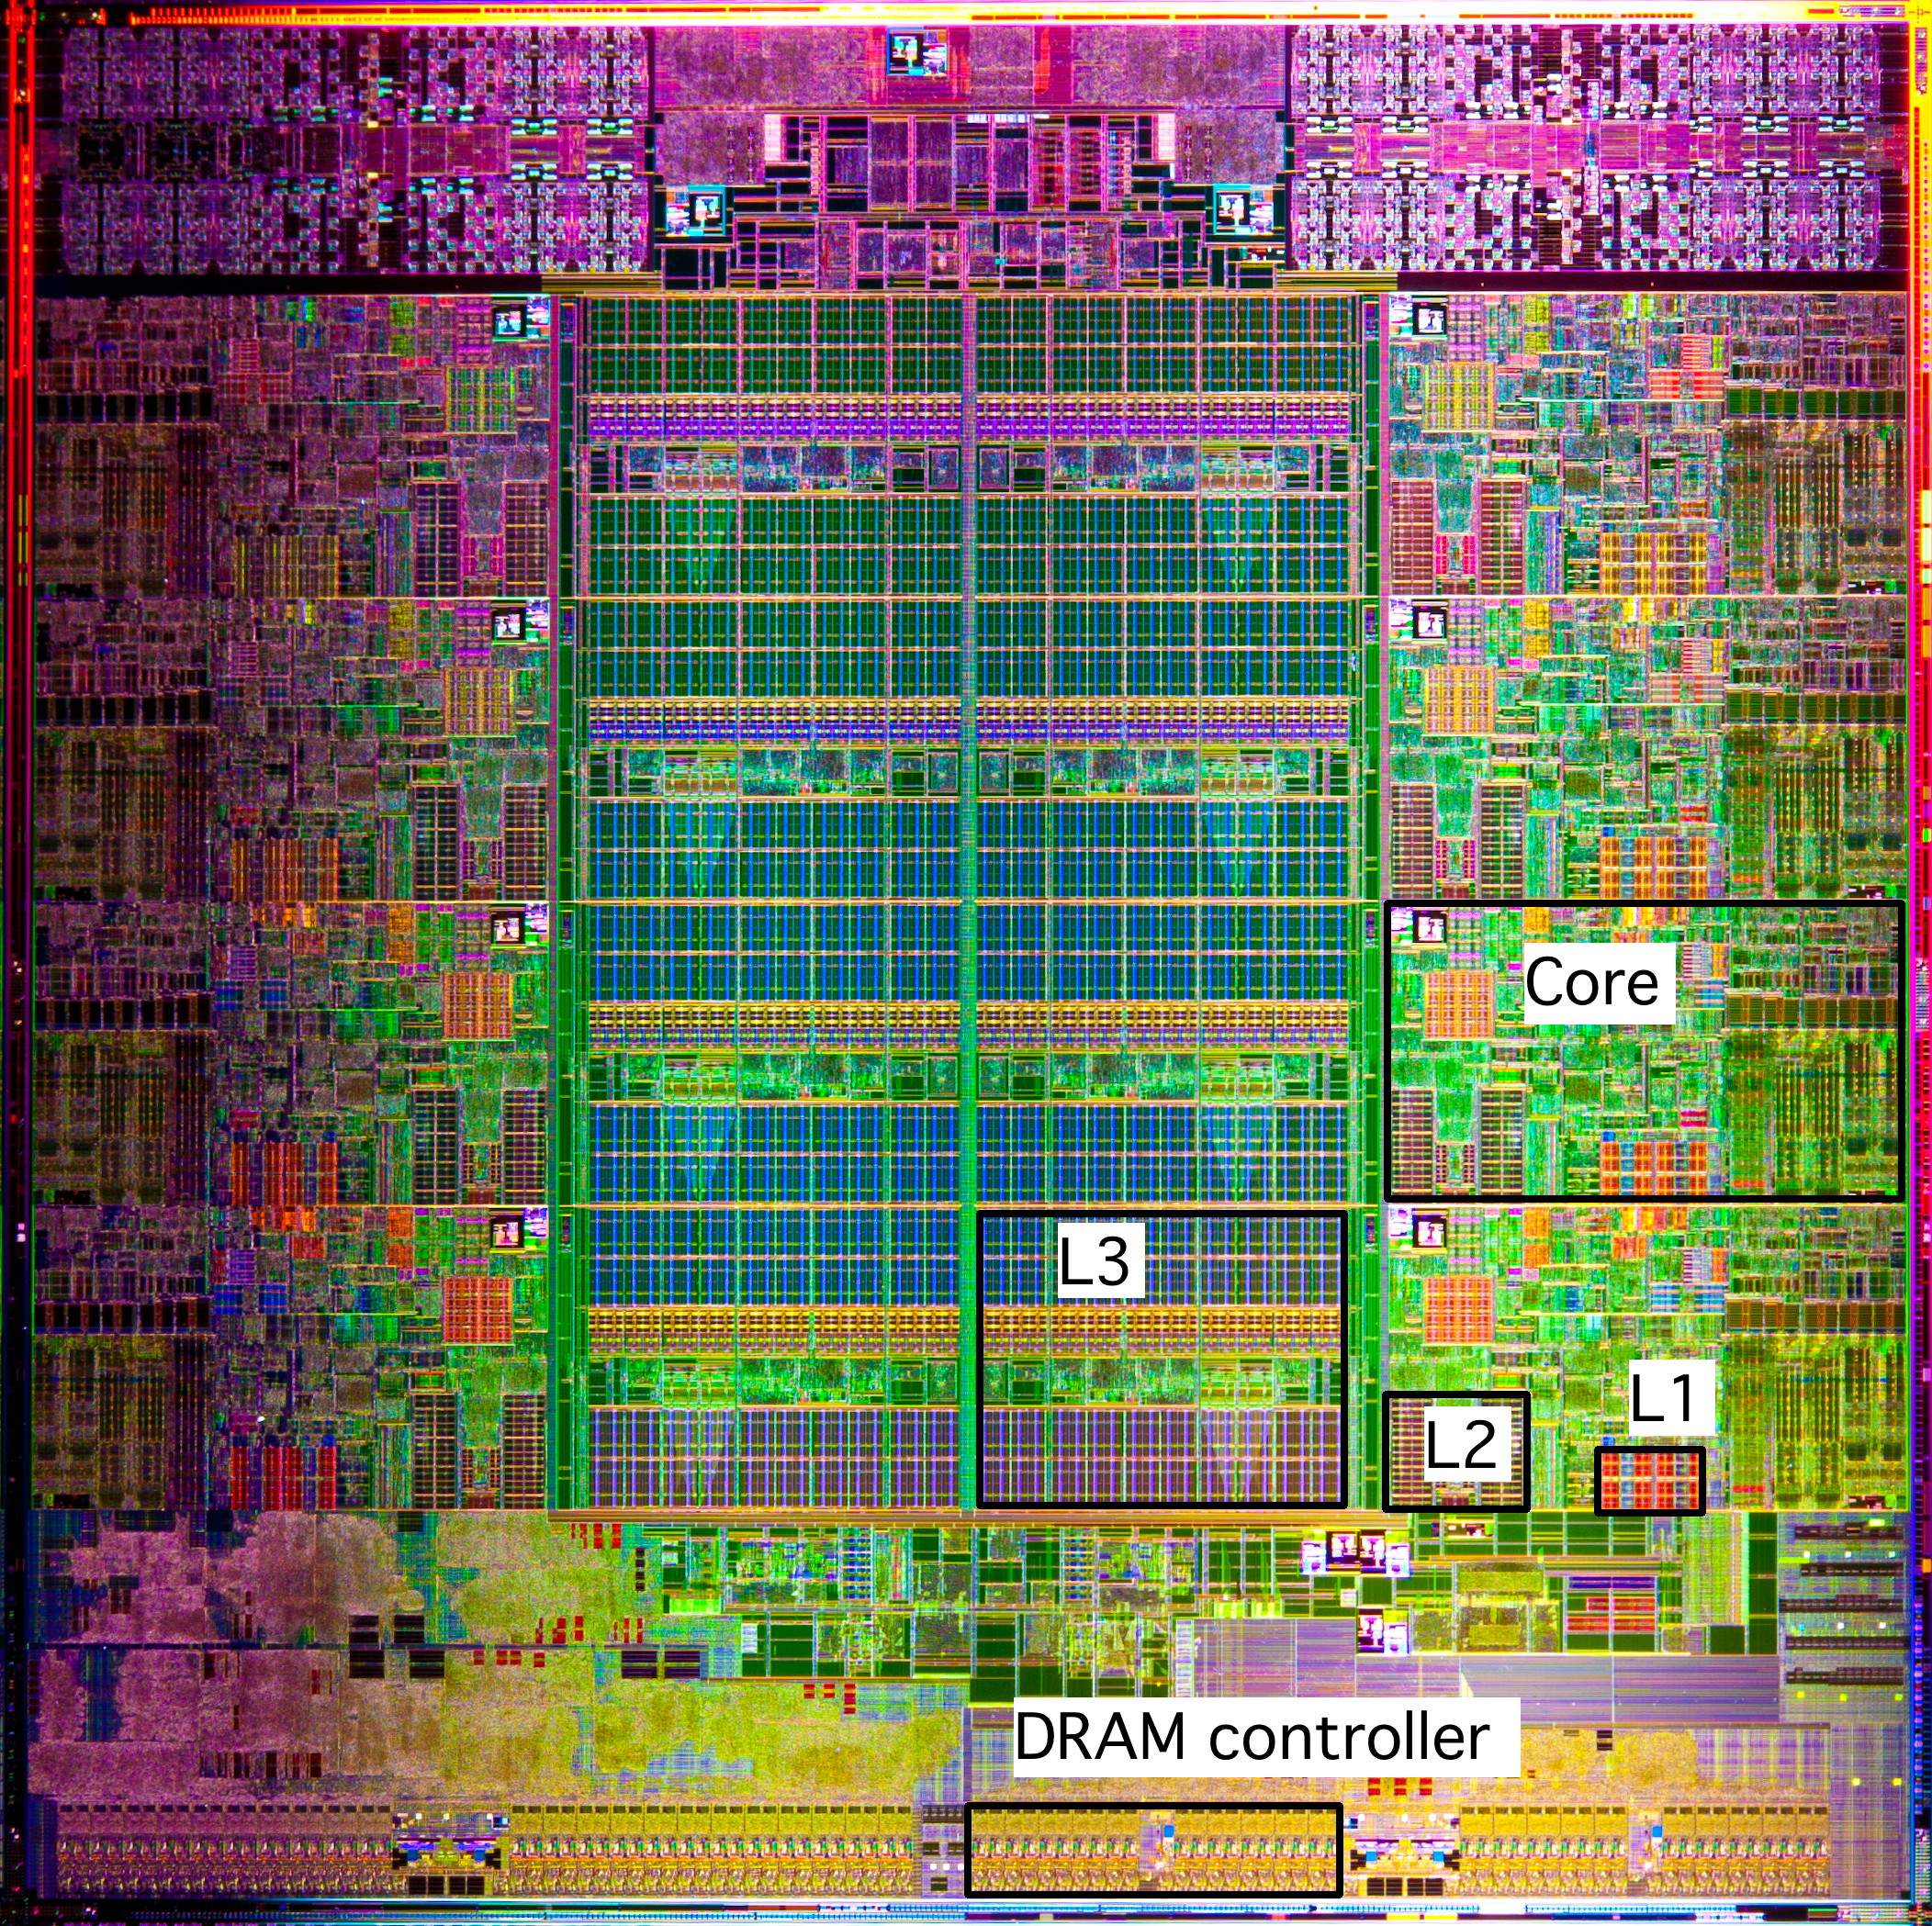
\includegraphics[scale=.45]{sandybridge-eightcore-ann}
  \caption{The Intel Sandybridge processor die}
  \label{fig:sandybridge}
\end{wrapfigure}

\Level 2 {Instruction handling}

\index{out-of-order|see{instruction, handling, out-of-order}} The Von
Neuman model is also unrealistic in that it assumes that all
instructions are executed strictly in sequence.  Increasingly, over
the last twenty years, processor have used
\emph{out-of-order}\index{instruction!handling!out-of-order}
instruction handling, where instructions can be processed
in a different order than the user program specifies. 
Of course the processor is only allowed to re-order instructions
if that leaves the result of the execution intact!

In the block diagram (figure~\ref{fig:sandycore}) you see various
units that are concerned with instrunction handling: This cleverness
actually costs considerable energy, as well as sheer amount of
transistors. For this reason, processors such as the
\indextermbus{Intel}{Xeon Phi} use
\emph{in-order}\index{instruction!handling!in-order} instruction
handling.

\Level 2 {Floating point units}
\index{floating point!unit|(textbf}

In scientific computing we are mostly interested in what a processor
does with floating point data. Computing with integers or booleans 
is typically of less interest. For this reason, cores have
considerable sophistication for dealing with numerical data.

For instance, while past processors had just a single \acf{FPU},
these days they will have multiple, capable of executing
simultaneously.

For instance, often there are separate addition and
multiplication units; if the compiler can find addition and
multiplication operations that are independent, it can schedule them
so as to be executed simultaneously, thereby doubling the performance
of the processor. In some cases, a processor will have multiple
addition or multiplication units.

Another way to increase performance is to have a \indexacf{FMA}
unit, which can execute the instruction $x\leftarrow ax+b$ in the same
amount of time as a separate addition or multiplication. Together with
pipelining (see below), this means that a processor has an asymptotic
speed of several floating point operations per clock cycle.

\begin{figure}[ht]
  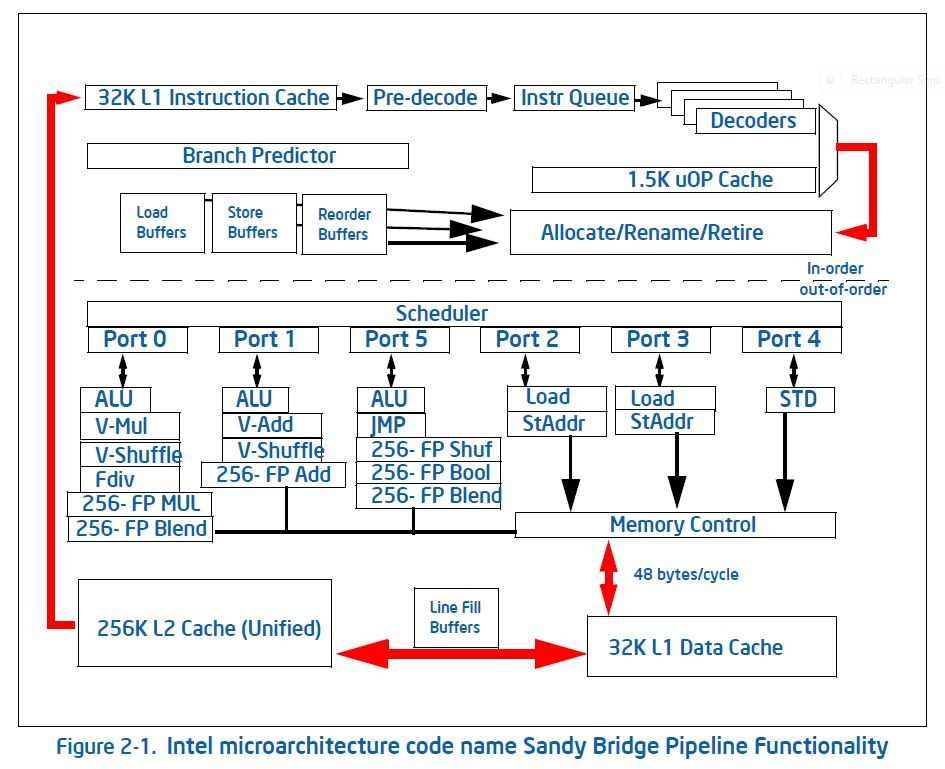
\includegraphics[scale=.6]{sandybridge_pipeline}
  \caption{Block diagram of the Intel Sandy Bridge core}
  \label{fig:sandycore}
\end{figure}

\begin{table}[h]
  \index{Intel!Sandy Bridge}\index{Intel!Haswell}\index{DEC!Alpha}\index{IBM!Power 5}
  \centering
  \begin{tabular}{p{2in}llll}
Processor&year&add/mult/fma units  &daxpy cycles\\
         &    &(count$\times$width)&(arith vs load/store)\\
\hline
MIPS R10000       &1996 &$1\times1+1\times1+0$ &8/24 \\
Alpha EV5         &1996 &$1\times1+1\times1+0$ &8/12 \\
IBM Power5        &2004 &$0+0+2\times1       $ &4/12 \\
AMD Bulldozer     &2011 &$2\times2+2\times2+0$ &2/4  \\
Intel Sandy Bridge&2012 &$1\times4+1\times4+0$ &2/4  \\
Intel Haswell     &2014 &$0+0+2\times 4      $ &1/2  \\
%Intel Woodcrest, AMD Barcelona&2 add + 2 mul&4 \\  %SIMD FADD, FMUL
%IBM POWER4, POWER5, POWER6&    2 FMA & 4 \\
%IBM BG/L, BG/P & 1 SIMD FMA & 4 \\
%SPARC IV & 1 add + 1 mul& 2 \\
%Itanium2 &  2 FMA & 4 
  \end{tabular}
  \caption{Floating point capabilities (per core) of several processor architectures,
  and DAXPY cycle number for 8 operands}
  \label{tab:chipfloats}
\end{table}

Incidentally, there are few algorithms in which division operations
are a limiting factor. Correspondingly, the division operation is not
nearly as much optimized in a modern CPU as the additions and
multiplications are. Division operations can take 10 or 20 clock
cycles, while a CPU can have multiple addition and/or multiplication
units that (asymptotically) can produce a result per cycle.

\index{floating point!unit|)textbf}

\Level 2 {Pipelining}
\label{sec:pipeline}
\index{pipeline|(textbf}

The floating point add and multiply units of a processor are
pipelined, which has the effect that a stream of independent
operations can be performed at an asymptotic speed of one result per
clock cycle.

\input chapters/pipeline

\index{pipeline|)}

\Level 2 {Peak performance}

Thanks to pipelining, for modern CPUs there is a simple relation
between the \indexterm{clock speed} and the \indexterm{peak performance}.
Since each \ac{FPU} can produce one result per cycle
asymptotically, the peak performance is the clock speed times the
number of independent \acp{FPU}. The measure of floating
point performance is `floating point operations per second',
abbreviated \indexterm{flops}. Considering the speed of computers
these days, you will mostly hear floating point performance being
expressed in `gigaflops': multiples of $10^9$ flops.

\Level 1 {8-bit, 16-bit, 32-bit, 64-bit}

Processors are often characterized in terms of how big a chunk of data
they can process as a unit. This can relate to
\begin{itemize}
\item The width of the path between processor and memory: can a 64-bit
  floating point number be loaded in one cycle, or does it arrive in
  pieces at the processor.
\item The way memory is addressed: if addresses are limited to 16
  bits, only 64,000 bytes can be identified. Early PCs had a
  complicated scheme with segments to get around this limitation: an
  address was specified with a segment number and an offset inside the segment.
% how did the Motorola 68k do this?
\item The number of bits in a register, in particular the size of the
  integer registers which manipulate data address; see the previous
  point. (Floating point register are often larger, for instance 80
  bits in the x86 architecture.) This also corresponds to the size of
  a chunk of data that a processor can operate on simultaneously.
\item The size of a floating point number. If the arithmetic unit of a
  CPU is designed to multiply 8-byte numbers efficiently (`double
  precision'; see section~\ref{sec:float-representation}) then numbers half
  that size (`single precision') can sometimes be processed at higher
  efficiency, and for larger numbers (`quadruple precision') some
  complicated scheme is needed. For instance, a quad precision number
  could be emulated by two double precision numbers with a fixed
  difference between the exponents.
\end{itemize}
These measurements are not necessarily identical. For instance, the
original Pentium processor had 64-bit data busses, but a 32-bit
processor. On the other hand, the Motorola 68000 processor (of the
original Apple Macintosh) had a 32-bit CPU, but 16-bit data busses.

The first Intel\index{Intel} microprocessor, the 4004, was a 4-bit
processor in the sense that it processed 4 bit chunks. These days,
64 bit processors are becoming the norm.

\Level 1 {Caches: on-chip memory}

The bulk of computer memory is in chips that are separate from the processor.
However, there is usually a small amount (typically a few megabytes)
of on-chip memory, called the \indexterm{cache}. This will be 
explained in detail in section~\ref{sec:cache}.

\Level 1 {Graphics, controllers, special purpose hardware}

One difference between `consumer' and `server' type processors
is that the consumer chips devote considerable real-estate
on the processor chip to graphics. Processors for cell phones and tablets
can even have dedicated circuitry for security or mp3 playback.
Other parts of the processor
are dedicated to communicating with memory or the \indexterm{I/O subsystem}.
We will not discuss those aspects in this book.

\Level 1 {Superscalar processing and instruction-level parallelism}
\label{sec:pipelinecpu}

In the von Neumann model processors operate through \indextermdef{control flow}:
instructions follow each other linearly or with branches without regard for what
data they involve. As processors became more powerful and capable of executing
more than one instruction at a time, it became necessary to switch to the
\indextermdef{data flow} model. Such \indextermdef{superscalar} processors
analyze several instructions to find data dependencies, and execute
instructions in parallel that do not depend on each other.

This concept is also known as \indexacf{ILP}, and it is facilitated by
various mechanisms:
\begin{itemize}
\item multiple-issue: instructions that are independent can be started
  at the same time;
\item pipelining: already mentioned, arithmetic units can deal with
  multiple operations in various stages of completion;
\item branch prediction and speculative execution: a compiler can
  `guess' whether a conditional instruction will evaluate to true, and
  execute those instructions accordingly;
\item out-of-order execution: instructions can be rearranged if they
  are not dependent on each other, and if the resulting execution will
  be more efficient;
\item prefetching: data can be speculatively requested before any
  instruction needing it is actually encountered (this is discussed
  further in section~\ref{sec:prefetch}).
\end{itemize}

Above, you saw pipelining in the context of floating point
operations. Nowadays, the whole CPU is pipelined. Not only floating point
operations, but any sort of instruction will be put in the
\indextermbus{instruction}{pipeline} as soon
as possible. Note that this pipeline is no longer limited to identical
instructions: the notion of pipeline is now generalized to any stream
of partially executed instructions that are simultaneously ``in
flight''.

As clock frequency has gone up, the processor pipeline has grown in
length to make the segments executable in less time. You have already
seen that longer pipelines have a larger $n_{1/2}$, so more
independent instructions are needed to make the pipeline run at full
efficiency. As the limits to instruction-level parallelism are
reached, making pipelines longer\index{pipeline!length} (sometimes
called `deeper'\index{pipeline!depth}) no longer pays off. This is
generally seen as the reason that chip designers have moved to
\indexterm{multicore} architectures as a way of more efficiently
using the transistors on a chip; section~\ref{sec:multicore}.

There is a second problem with these longer pipelines: if the code
comes to a branch point (a conditional or the test in a loop), it is
not clear what the next instruction to execute is. At that point the
pipeline can \emph{stall}\index{pipeline!stall}. CPUs have taken to
\indexterm{speculative execution} for instance, by always assuming
that the test will turn out true. If the code then takes the other
branch (this is called a \indexterm{branch misprediction}), the
pipeline has to be \emph{flushed}\index{pipeline!flush} and
restarted. The resulting delay in the execution stream is called the
\indexterm{branch penalty}.

\Level 0 {Memory Hierarchies}
\label{sec:hierarchy}

We will now refine the picture of the Von Neuman architecture, in
which data is loaded immediately from memory to the processors, where
it is operated on. This picture is unrealistic because of the
so-called \indextermbus{memory}{wall}~\cite{Wulf:memory-wall}: the
memory is too slow to load data into the process at the rate the
processor can absorb it. Specifically, a single load can take 1000
cycles, while a processor can perform several operations per
cycle. (After this long wait for a load, the next load can come
faster, but still too slow for the processor. This matter of wait time
versus throughput will be addressed below in
section~\ref{sec:latencybandwidth}.)

In reality, there will be various memory levels in between the
\ac{FPU} and the main memory: the registers\index{register}
and the caches\index{cache}, together called the
\indextermbus{memory}{hierarchy}. These try to alleviate the memory
wall problem by making recently used data available quicker than it
would be from main memory. Of course, this presupposes that the
algorithm and its implementation allow for data to be used multiple
times.  Such questions of \indexterm{data reuse} will be discussed in
more detail in section~\ref{sec:reuse}.

Both registers and caches are faster
than main memory to various degrees; unfortunately, the faster the memory on a certain
level, the smaller it will be.
These differences in size and access speed lead to interesting programming
problems, which we will discuss later in this chapter, and
particularly section~\ref{sec:performance-programming}.

We will now discuss the various components of the memory hierarchy and
the theoretical concepts needed to analyze their behaviour.

\Level 1 {Busses}

The wires that move data around in a computer, from memory to cpu or
to a disc controller or screen, are called \emph{busses}\index{bus}. The
most important one for us is the \indexac{FSB} which connects the processor to memory. In one popular
architecture, this is called the `north bridge', as opposed to the
`south bridge' which connects to external devices, with the exception
of the graphics controller.

\begin{figure}[ht]
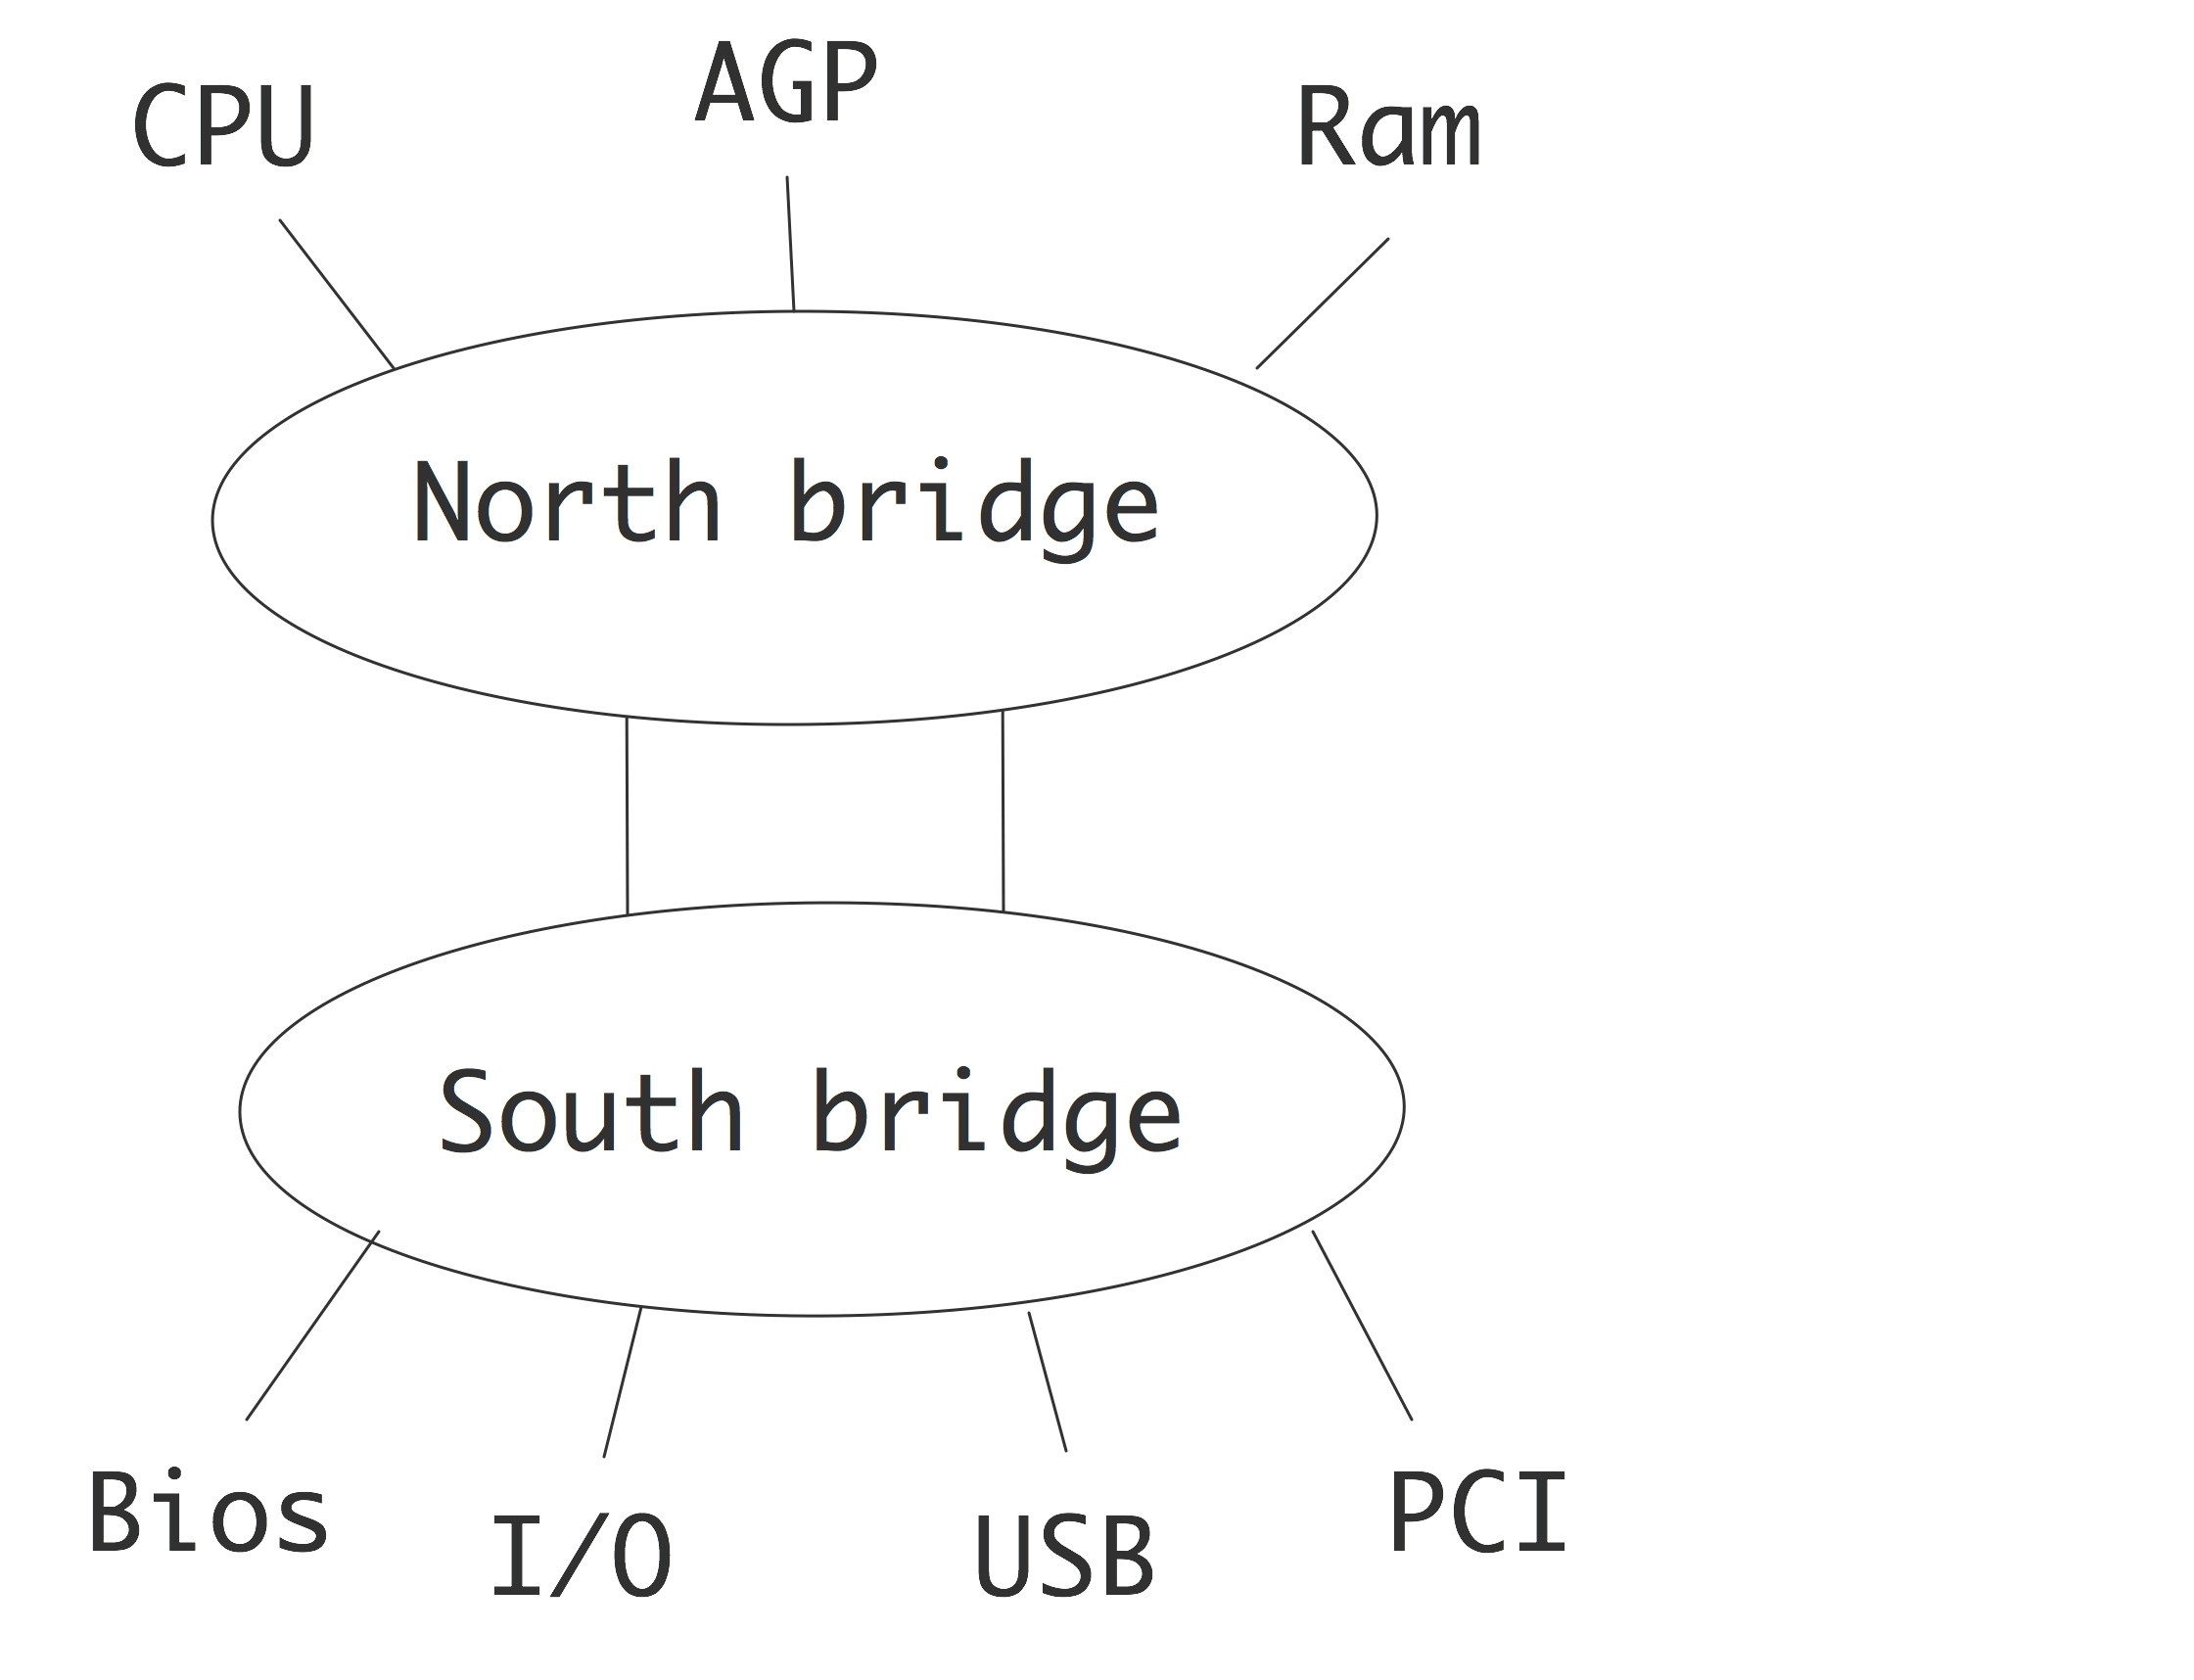
\includegraphics[scale=.1]{graphics/bridges}
\caption{Bus structure of a processor}
\end{figure}

The bus is typically slower than the processor, operating with clock
frequencies slightly in excess of~1GHz, which is a fraction of the CPU
clock frequency.  This is one reason that caches are needed; the fact
that a processors can consume many data items per clock tick
contributes to this. Apart from the frequency, the bandwidth of a bus is
also determined by the number of bits that can be moved per clock
cycle. This is typically 64 or 128 in current architectures. We will
now discuss this in some more detail.

\Level 1 {Latency and Bandwidth}
\label{sec:latencybandwidth}

Above, we mentioned in very general terms that accessing data in
registers is almost instantaneous, whereas loading data from memory
into the registers, a necessary step before any operation, incurs a
substantial delay. We will now make this story slightly more precise.

There are two important concepts to describe the movement of data:
\indexterm{latency} and \indexterm{bandwidth}. The assumption here is
that requesting an item of data incurs an initial delay; if this item
was the first in a stream of data, usually a consecutive range of
memory addresses, the remainder of the stream will arrive with no
further delay
at a regular amount per time period.
\begin{description}
\item[Latency] is the delay between the processor issuing a request
  for a memory item, and the item actually arriving. We can
  distinguish between various latencies, such as the transfer from
  memory to cache, cache to register, or summarize them all into the
  latency between memory and processor. Latency is measured in (nano)
  seconds, or clock periods.

  If a processor executes instructions in the order they are found in
  the assembly code, then execution will often \emph{stall}\index{stall|see{memory!stall}} while
  data is being fetched from memory; this is also called
  \indextermbus{memory}{stall}. For this reason, a low latency is very
  important. In practice, many processors have `out-of-order
  execution' of instructions, allowing them to perform other
  operations while waiting for the requested data. Programmers can
  take this into account, and code in a way that achieves
  \indextermbus{latency}{hiding}; see also section~\ref{sec:intensity}.
  \acp{GPU} 
\begin{gpu}
  (see section~\ref{sec:gpu})  
\end{gpu}
  can switch very quickly between threads in order to achieve latency hiding.
\item[Bandwidth] is the rate at which data arrives at its destination,
  after the initial latency is overcome. Bandwidth is measured in
  bytes (kilobyes, megabytes, gigabyes) per second or per clock cycle.
  The bandwidth between two memory levels is usually the product of
  the cycle speed of the channel (the \indextermbus{bus}{speed}) and
  the \indextermbus{bus}{width}: the number of bits that can be sent
  simultaneously in every cycle of the bus clock.
\end{description}

The concepts of latency and bandwidth are often combined in a formula
for the time that a message takes from start to finish:
\[ T(n) = \alpha+\beta n \]
where $\alpha$ is the latency and $\beta$ is the inverse of the
bandwidth: the time per byte.

Typically, the further away from the processor one gets, the longer
the latency is, and the lower the bandwidth.
These two factors make it important to program in such a
way that, if at all possible, the processor uses data from cache or register,
rather than from main memory. To illustrate that this is a serious
matter, consider a vector addition
\begin{verbatim}
for (i)
  a[i] = b[i]+c[i]
\end{verbatim}
Each iteration performs one floating point operation, which modern
CPUs can do in one clock cycle by using pipelines. However, each
iteration needs two numbers loaded and one written, for a total of 24
bytes\footnote{Actually, \n{a[i]} is loaded before it can be written,
so there are 4 memory access, with a total of 32 bytes, per
iteration.} of memory traffic. Typical memory bandwidth figures (see
for instance figure~\ref{fig:hierarchy}) are nowhere near 24 (or~32) bytes per
cycle. This means that, without caches, algorithm performance can be
bounded by memory performance. Of course, caches will not speed up
every operations, and in fact will have no effect on the above
example. Strategies for programming that lead to significant cache use
are discussed in section~\ref{sec:performance-programming}.

The concepts of latency and bandwidth will also appear in parallel
computers, when we talk about sending data from one processor to the
next.

\Level 1 {Registers}
\label{sec:register}
\index{register|(textbf}

Every processor has a small amount of memory that is internal to the
processor: the \emph{registers}, or together the
\indextermbus{register}{file}. The registers are what the processor
actually operates on: an operation such as 
\begin{verbatim}
a := b + c
\end{verbatim}
is actually implemented as 
\begin{itemize}
\item load the value of \n{b} from memory into a register,
\item load the value of \n{c} from memory into another register,
\item compute the sum and write that into yet another register, and
\item write the sum value back to the memory location of~\n{a}.
\end{itemize}
Looking at assembly code (for instance the output of a compiler), you
see the explicit load, compute, and store instructions.

Compute instructions such as add or multiply only operate on
registers. For instance, in \indextermbus{assembly}{language}
you will see instructions such as
\begin{verbatim}
addl	%eax, %edx
\end{verbatim}
which adds the content of one register to
another. As you see in this sample instruction, registers are not
numbered, as opposed to memory addresses,
but have distinct names that are referred to in
the assembly instruction. Typically, a processor has 16 or 32
floating point registers; the \indextermbus{Intel}{Itanium} was
exceptional with 128 floating point registers.

Registers have a high bandwidth and low latency because they
are part of the processor. You can consider data movement to and from
registers as essentially instantaneous.

In this chapter you will see stressed that moving data from memory is
relatively expensive. Therefore, it would be a simple optimization to
leave data in register when possible. For instance, if the above
computation is followed by a statement
\begin{verbatim}
a := b + c
d := a + e
\end{verbatim}
the computed value of \n{a} could be left in register. This
optimization is typically performed as a
\indextermbus{compiler}{optimization}: the compiler will simply not
generate the instructions for storing and reloading~\n{a}. We say that
\n{a} stays \indextermsub{resident in}{register}.

Keeping values in register is often done to avoid recomputing a
quantity. For instance, in 
\begin{verbatim}
t1 = sin(alpha) * x + cos(alpha) * y;
t2 = -cos(alsph) * x + sin(alpha) * y;
\end{verbatim}
the sine and cosine quantity will probably be kept in register. You
can help the compiler by explicitly introducing temporary quantities:
\begin{verbatim}
s = sin(alpha); c = cos(alpha);
t1 = s * x + c * y;
t2 = -c * x + s * y
\end{verbatim}
Of
course, there is a limit to how many quantities can be kept in
register; trying to keep too many quantities in register is called
\indextermbus{register}{spill} and lowers the performance of a code.

Keeping a variable in register is especially important if that
variable appears in an inner loop. In the computation
\begin{verbatim}
for i=1,length
  a[i] = b[i] * c
\end{verbatim}
the quantity \n{c} will probably be kept in register by the compiler,
but in 
\begin{verbatim}
for k=1,nvectors
  for i=1,length
    a[i,k] = b[i,k] * c[k]
\end{verbatim}
it is a good idea to introduce explicitly a temporary variable to
hold~\n{c[k]}. In~C, you can give a hint to the compiler
to keep a veriable in register by declaring it as a \indextermbus{register}{variable}:
\begin{verbatim}
register double t;
\end{verbatim}

\index{register|)}

\Level 1 {Caches}
\label{sec:cache}
\index{cache|(textbf}

In between the registers, which contain the immediate input and output
data for instructions, and the main memory where lots of data can reside for a
long time, are various levels of \emph{cache} memory, that have
lower latency and higher bandwidth than main memory and where data are
kept for an intermediate amount of time.  Caches typically
consist of \indexac{SRAM}, which is faster than then \indexac{DRAM}
used for the main memory, but is also more expensive.

Data from
memory travels through the caches to wind up in registers. The
advantage to having cache memory is that if a data item is reused
shortly after it was first needed, it will still be in cache, and
therefore it can be accessed much faster than if it would have to be
brought in from memory.

\Level 2 {A motivating example}

As an example, let's suppose a variable \n{x} is used twice, and its
uses are too far apart that it would stay \indextermsub{resident
  in}{register}:
\begin{verbatim}
... = ... x ..... // instruction using x
.........         // several instructions not involving x
... = ... x ..... // instruction using x
\end{verbatim}
The assembly code would then be
\begin{itemize}
\item load \n{x} from memory into register; operate on it;
\item do the intervening instructions;
\item load \n{x} from memory into register; operate on it;
\end{itemize}
With a cache, the assembly code stays the same, but the actual
behaviour of the memory system now becomes:
\begin{itemize}
\item load \n{x} from memory into cache, and from cache into register;
  operate on it;
\item do the intervening instructions;
\item request \n{x} from memory, but since it is still in the cache,
  load it from the cache into register; operate on it.
\end{itemize}
Since loading from cache is faster than loading from main memoory, the
computation will now be faster. Caches are fairly small, so values
can not be kept there indefinitely. We will see the implications of
this in the following discussion.

There is an important difference between cache memory and registers:
while data is moved into register by explicit assembly instructions,
the move from main memory to cache is entirely done by hardware.  Thus
cache use and reuse is outside of direct programmer control. Later,
especially in sections \ref{sec:locality} and
~\ref{sec:performance-programming}, you will see how it is possible to
influence cache use indirectly.

\Level 2 {Cache levels, speed and size}
\label{sec:cache-level}

The caches are called `level~1' and `level~2' (or, for short, L1 and
L2) cache; some processors can have an L3 cache.  The L1 and L2 caches
are part of the \indexterm{die}, the processor chip, although for the
L2 cache that is a relatively recent development; the L3 cache is
off-chip.  The L1 cache is small, typically around 16Kbyte. Level~2
(and, when present, level~3) cache is more plentiful, up to several
megabytes, but it is also slower.  Unlike main memory, which is
expandable, caches are fixed in size. If a version of a processor chip
exists with a larger cache, it is usually considerably more expensive.

Data needed in some operation gets copied into the various
caches on its way to the processor. If, some instructions later, a
data item is needed again, it is first searched for in the L1 cache; if it is
not found there, it is searched for in the L2 cache; if it is not found there,
it is loaded from main memory. Finding data in cache is called a
\indextermbus{cache}{hit}, and not finding it a \indextermbus{cache}{miss}.

Figure \ref{fig:hierarchy} illustrates the basic facts of the
\indextermbus{cache}{hierarchy}, in
this case for the \indextermbus{Intel}{Sandy Bridge} chip: the
closer caches are to the \acp{FPU}, the faster, but also the
smaller they are.
\begin{figure}[ht]
  \begin{quote}
  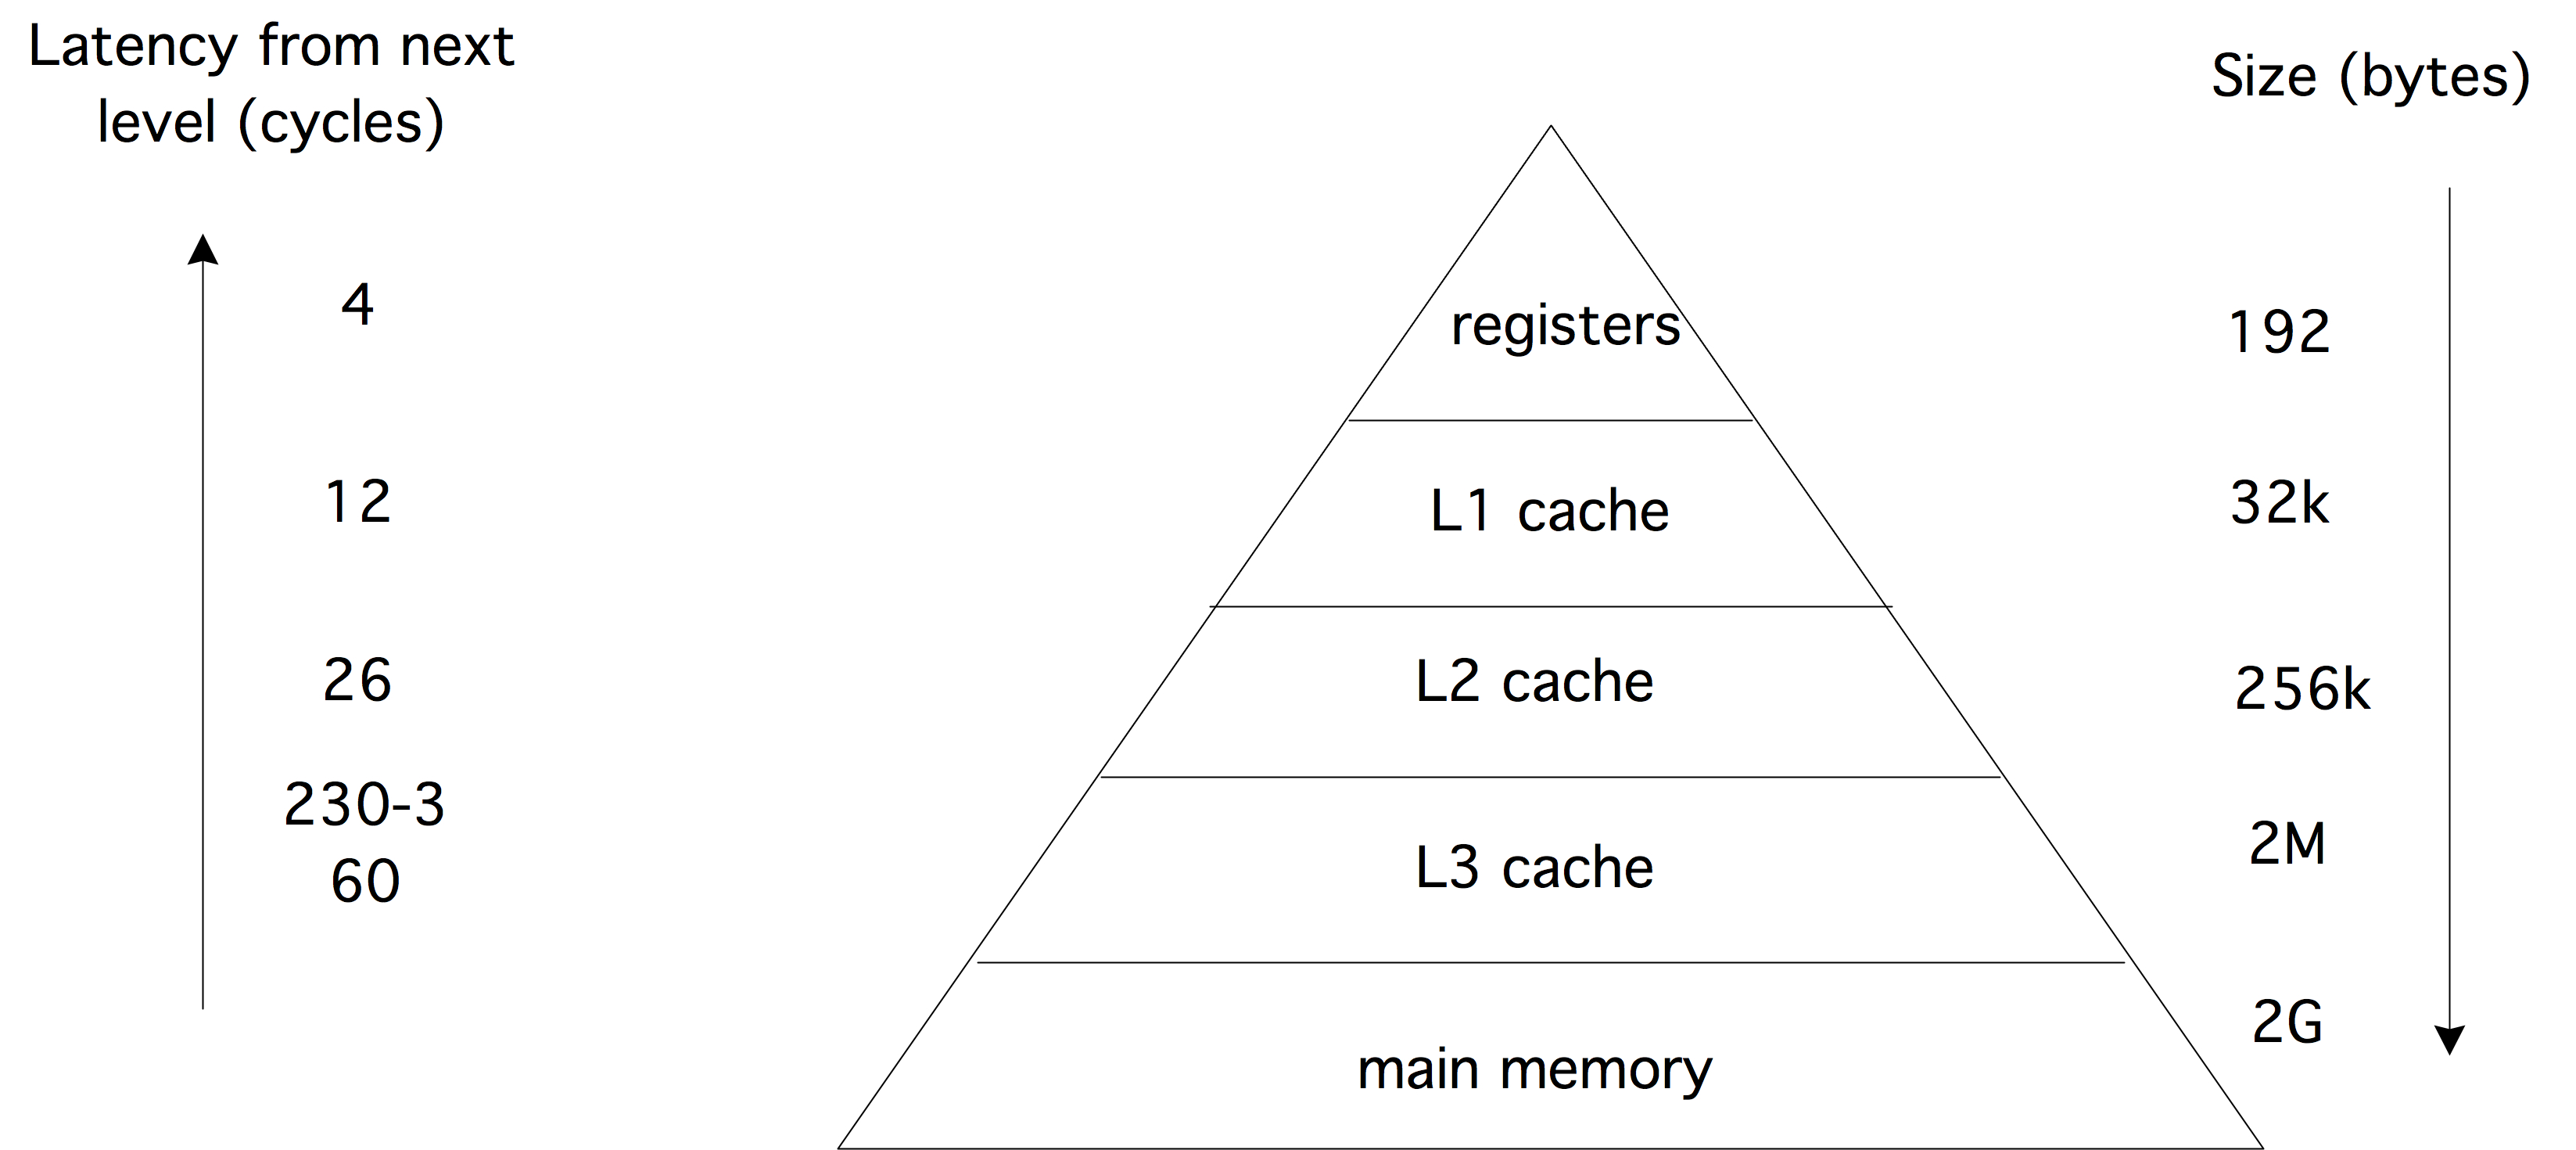
\includegraphics[scale=.11]{graphics/hierarchysb}
  \end{quote}
  \caption{Memory hierarchy of an Intel Sandy Bridge, characterized by speed and size.}
  \label{fig:hierarchy}
\end{figure}
Some points about this figure.
\begin{itemize}
\item Loading data from registers is so fast that it does not
  constitute a limitation on algorithm execution speed. On the other
  hand, there are few registers. Each core has 16 general purpose
  registers, and 16 SIMD registers.
\item The L1 cache is small, but sustains a bandwidth of 32 bytes,
  that is 4 double precision number, per cycle. This is enough to load
  two operands each for two operations, but note that the core can
  actually perform 4 operations per cycle. Thus, to achieve peak
  speed, certain operands need to stay in register: typically, L1 
  bandwidth is enough for about half of peak performance.
\item The bandwidth of the L2 and L3 cache is nominally the same as
  of L1. However, this bandwidth is partly wasted on coherence issues.
\item Main memory access has a latency of more than 100 cycles, and a
  bandwidth of 4.5 bytes per cycle, which is about $1/7$th of the L1
  bandwidth. However, this bandwidth is shared by the multiple cores
  of a processor chip, so effectively the bandwidth is a fraction of
  this number. Most clusters will also have more than one
  \indexterm{socket} (processor chip) per node, typically 2~or~4, so
  some bandwidth is spent on maintaining
  \indextermbus{cache}{coherence} (see section~\ref{sec:multicore}),
  again reducing the bandwidth available for each chip.
\end{itemize}

On level~1, there are separate caches for instructions and data; the
L2 and L3 cache contain both data and instructions.

You see that the larger caches are increasingly unable to supply data
to the processors fast enough. For this reason it is necessary to code
in such a way that data is kept as much as possible in the highest
cache level possible. We will discuss this issue in detail in the rest
of this chapter.

\begin{exercise}
  The L1 cache is smaller than the L2 cache, and if there is an L3,
  the L2 is smaller than the L3. Give a practical and a theoretical
  reason why this is so.  
\end{exercise}

\Level 2 {Types of cache misses}
\label{sec:cache-miss}

There are three types of cache misses.

As you saw in the example above, the first time you reference data you
will always incur a cache miss. This is known as a \emph{compulsory
cache miss}\index{cache!miss, compulsory} since these are unavoidable.
Does that mean that you will always be waiting for a data item, the first
time you need it? Not necessarily: section~\ref{sec:prefetch} explains
how the hardware tries to help you by predicting what data is needed next.

The next type of cache misses is due to the size of your working set:
a \emph{capacity cache miss}\index{cache!miss, capacity} is caused by
data having been overwritten because the cache can simply not contain
all your problem data. (Section~\ref{sec:lru} discusses how the processor
decides what data to overwrite.) If you want to avoid this type of misses, you
need to partition your problem in chunks that are small enough that
data can stay in cache for an appreciable time. Of course, this
presumes that data items are operated on multiple times, so that there
is actually a point in keeping it in cache; this is discussed in
section~\ref{sec:reuse}.

Finally, there are \emph{conflict misses}\index{cache!miss, conflict}
caused by one data item being mapped to the same cache location
as another, while both are still needed for the computation, and
there would have been better candidates to evict. This is discussed
in section~\ref{sec:associative}.

In a \indexterm{multicore} context there is a further type of cache miss:
the \emph{invalidation miss}\index{cache!miss, invalidation}. This happens
if an item in cache has become invalid because another core
changed the value of the corresponding memory address. The core will then
have to reload this address.

\Level 2 {Reuse is the name of the game}

The presence of one or more caches is not immediately a guarantee for
high performance: this largely depends on the \indextermbus{memory}{access
  pattern} of the code, and how well this exploits the caches.
The first time that an item is
referenced, it is copied from memory into cache, and through to the
processor registers. The latency and bandwidth for this are not mitigated in any
way by the presence of a cache. When the same item is referenced a
second time, it may be found in cache, at a considerably reduced cost
in terms of latency and bandwidth: caches have shorter latency and
higher bandwidth than main memory.

We conclude that, first, an algorithm has to have an opportunity for
data reuse. If every data item is used only once (as in addition of
two vectors), there can be no reuse, and the presence of caches is
largely irrelevant. A~code will only benefit from the increased
bandwidth and reduced latency of a cache if items in cache are
referenced more than once; see section~\ref{sec:reuse} for a detailed
discussion.. An example would be the matrix-vector multiplication
$y=Ax$ where each element of~$x$ is used in $n$ operations, where $n$
is the matrix dimension.

Secondly, an algorithm may theoretically
have an opportunity for reuse, but it needs to be coded in such a way
that the reuse is actually exposed. We will address these points in
section~\ref{sec:locality}. This second point especially is not
trivial.

Some problems are small enough that they fit completely in cache, at
least in the L3 cache. This is something to watch out for when
\indexterm{benchmarking}, since it gives a too rosy picture of
processor performance.

\Level 2 {Replacement policies}
\label{sec:lru}
\index{cache!replacement policies|(}

Data in cache and registers is placed there by the system, outside of
programmer control. Likewise, the system decides when to overwrite
data in the cache or in registers if it is not referenced in a while,
and as other data needs to be placed there.  Below, we will go into
detail on how caches do this, but as a general principle, a \acf{LRU}
cache replacement policy is used: if a cache is full and new data
needs to be placed into it, the data that was least recently used is
\indexterm{flushed}, meaning that it is overwritten with the new item,
and therefore no longer accessible. LRU is by far the most common
replacement policy; other possibilities are FIFO (first in first out)
or random replacement.

\begin{exercise}
  Sketch a simple scenario, and give some (pseudo) code, to argue that
  LRU is preferable over FIFO as a replacement strategy.
\end{exercise}

\index{cache!replacement policies|)}

\Level 2 {Cache lines}
\label{sec:cacheline}\label{sec:stride}
\index{cache!line|(}

Data movement between memory and cache, or between caches, is not done
in single bytes, or even words. Instead, the smallest unit of data
moved is called a \emph{cache line}, sometimes called a
\indextermbus{cache}{block}.  A~typical cache line is 64 or 128 bytes
long, which in the context of scientific computing implies 8 or 16
double precision floating point numbers. The cache line size for data
moved into L2 cache can be larger than for data moved into L1 cache.

It is important to acknowledge the existence of cache lines in coding,
since any memory access costs the transfer of several words (see
section~\ref{sec:coding-cacheline} for some examples). An
efficient program then tries to use the other items on the cache line,
since access to them is effectively free. This phenomenon is visible in
code that accesses arrays by \indexterm{stride}: elements are read or
written at regular intervals.

\begin{wrapfigure}{r}{3in}
  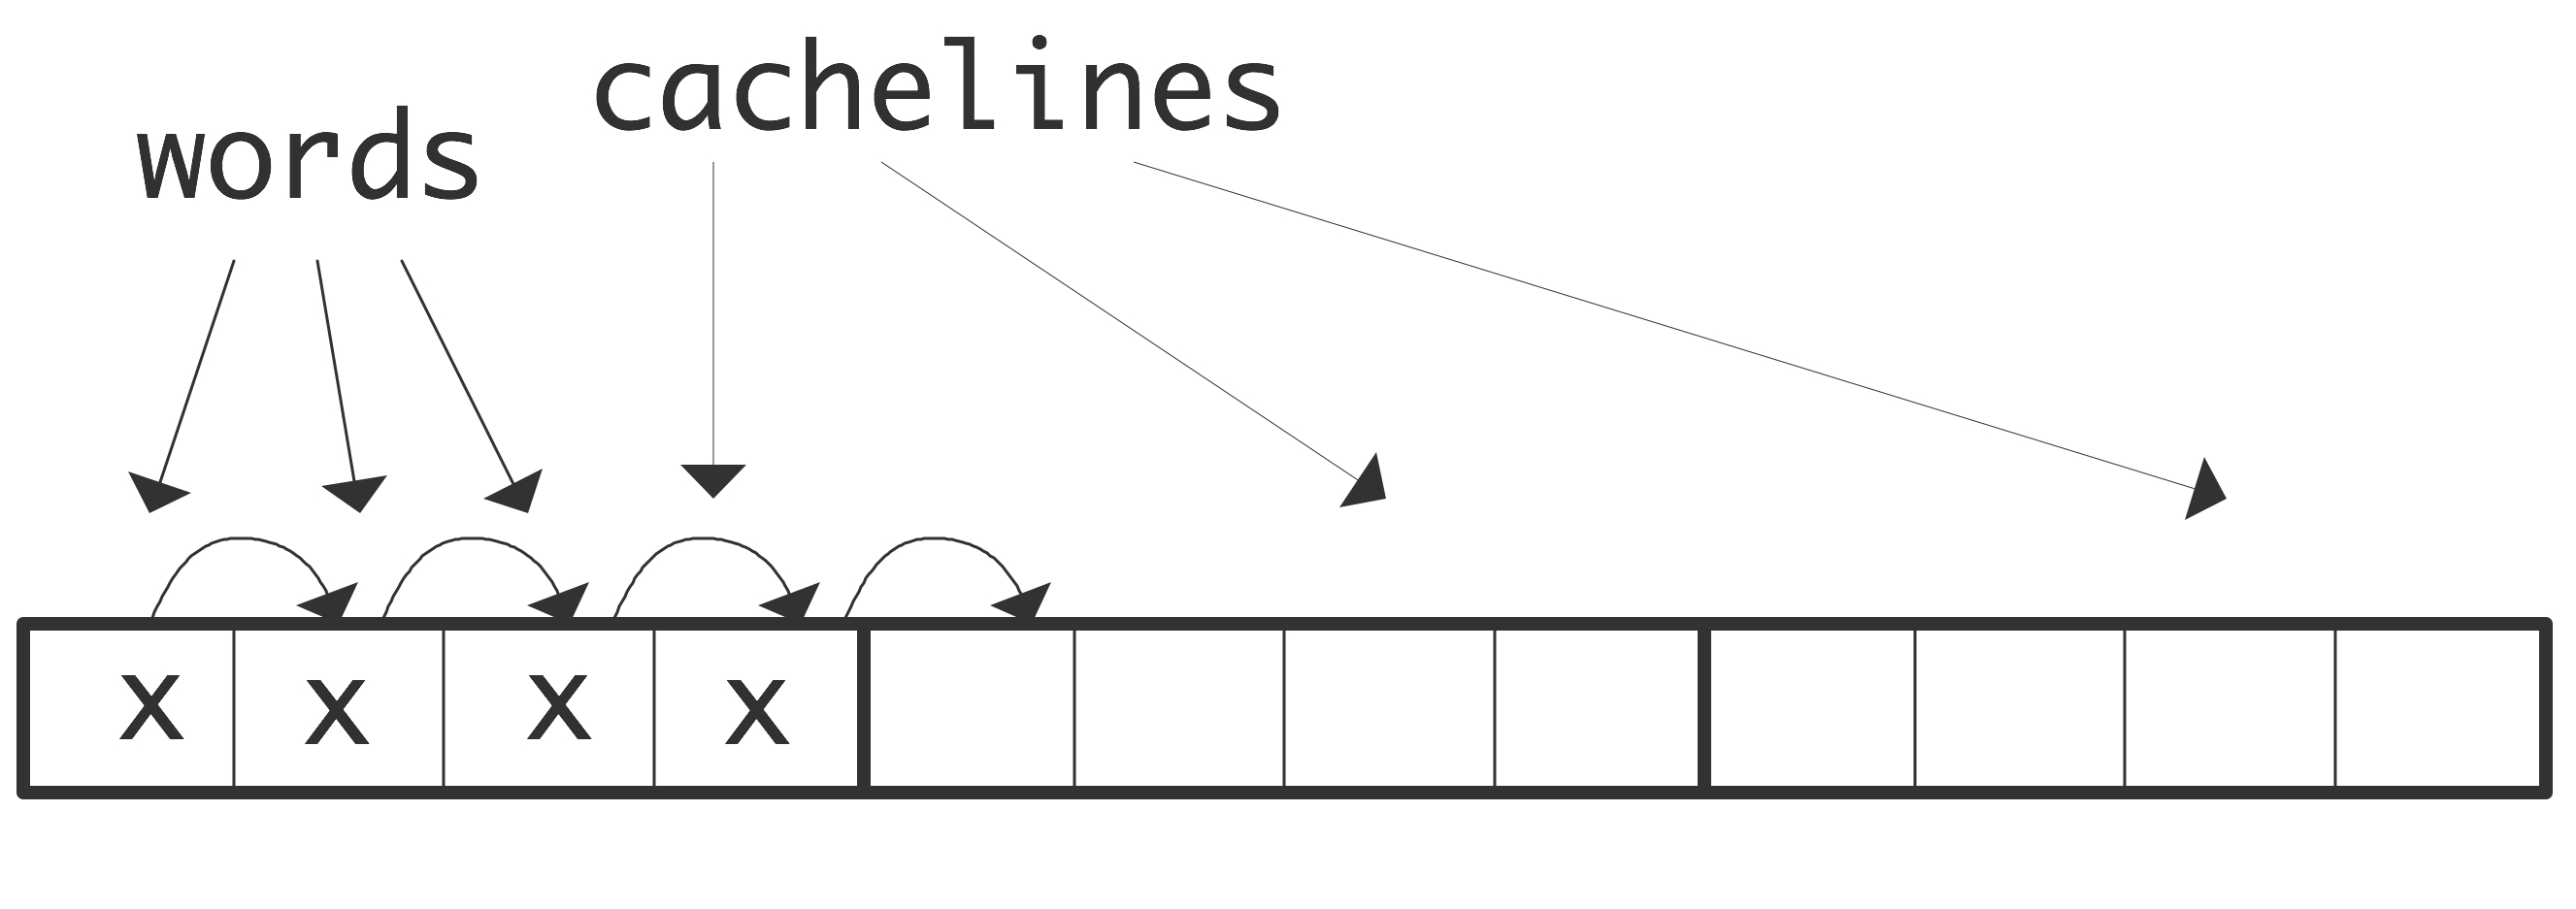
\includegraphics[scale=.07]{graphics/stride-1}
  \caption{Accessing 4 elements at stride 1}
  \label{fig:stride-1}
  \vskip-.5in
\end{wrapfigure}
%
Stride~1 corresponds to sequential access of an array:
\begin{verbatim}
for (i=0; i<N; i++)
  ... = ... x[i] ...
\end{verbatim}
Let us use as illustration a case with 4 words per cacheline. Requesting
the first elements loads the whole cacheline that contains it into
cache. A~request for the 2nd, 3rd, and 4th element can then be
satisfied from cache, meaning with high bandwidth and low latency.
\bigskip

\begin{wrapfigure}{r}{3in}
  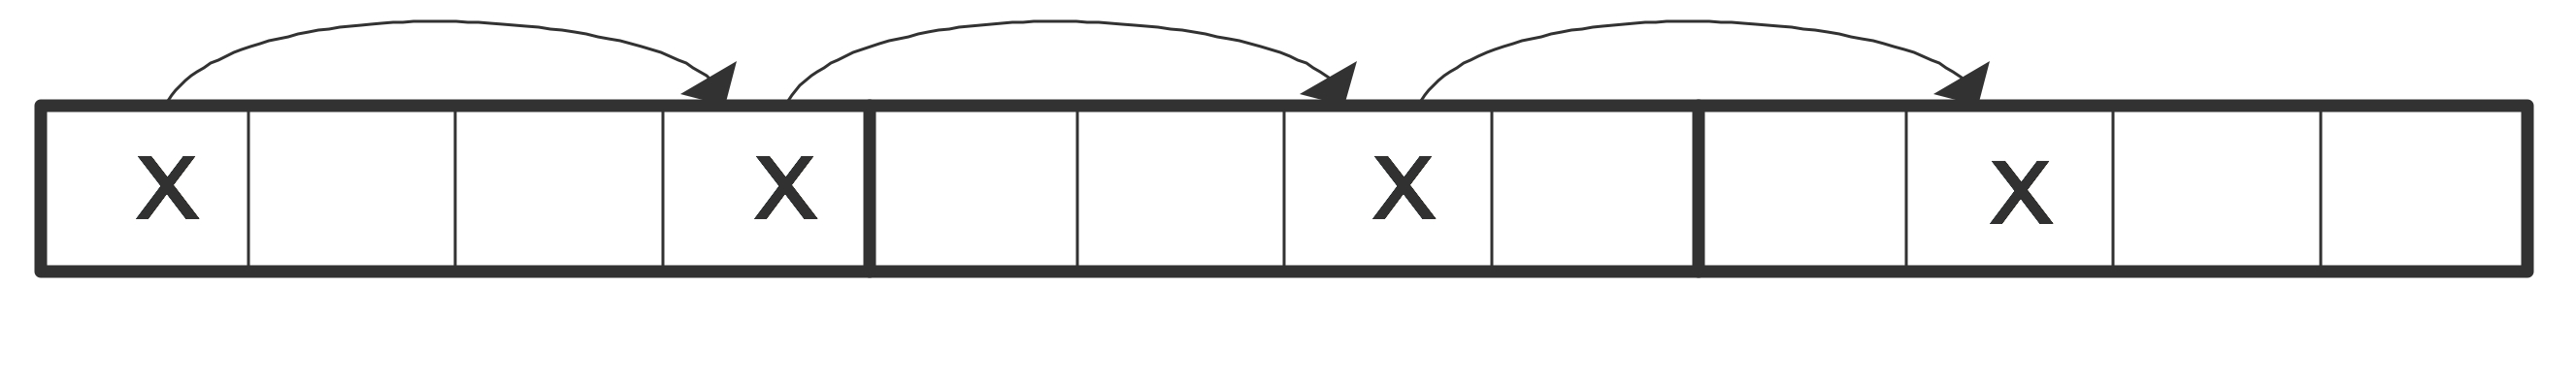
\includegraphics[scale=.07]{graphics/stride-3}
  \caption{Accessing 4 elements at stride 3}
  \label{fig:stride-3}
  \vskip-.5in
\end{wrapfigure}
%
A larger stride 
\begin{verbatim}
for (i=0; i<N; i+=stride)
  ... = ... x[i] ...
\end{verbatim}
implies that in every cache line only certain elements
are used. We illustrate that with stride~3: requesting the first
elements loads a cacheline, and this cacheline also contains the
second element. However, the third element is on the next cacheline,
so loading this incurs the latency and bandwidth of main memory. The
same holds for the fourth element. Loading four elements now needed
loading three cache lines instead of one, meaning that two-thirds of
the available bandwidth has been wasted. (This second case would also incur
three times the latency of the first, if it weren't for a hardware
mechanism that notices the regular access patterns, and pre-emtively
loads further cachelines; see section~\ref{sec:prefetch}.)

Some applications naturally lead to strides greater than~1, for
instance, accessing only the real parts of an array of complex
numbers (for some remarks on the practical realization of complex
numbers see section~\ref{sec:complex}). Also, methods that use
\indextermdef{recursive doubling} often have a code structure that
exhibits non-unit strides
\begin{verbatim}
for (i=0; i<N/2; i++)
  x[i] = y[2*i];
\end{verbatim}

In this discussion of cachelines, we have implicitly assumed the
beginning of a cacheline is also the beginning of a word, be that an
integer or a floating point number. This need not be true: an 8-byte
floating point number can be placed straddling the boundary between
two cachelines. You can image that this is not good for
performance. Section~\ref{sec:memalign} discusses ways to address
\indextermbus{cacheline}{boundary aligment}
in practice.

\index{cache!line|)}

\Level 2 {Cache mapping}

Caches get faster, but also smaller, the closer to the \acp{FPU} they
get, yet even the largest cache is considerably smaller than the main
memory size. We already noted that this has implications for the cache
replacement strategy. Another issue we need to address in this context
is that of \indextermbus{cache}{mapping}, which is the question of `if
an item is placed in cache, where does it get placed'. This problem is
generally addressed by mapping the (main memory) address of the item
to an address in cache, leading to the question `what if two items get
mapped to the same address'.

\Level 2 {Direct mapped caches}
\label{sec:directmap}

The simplest cache mapping strategy is \indexterm{direct
  mapping}. Suppose that memory addresses are 32 bits long, so that
they can address 4G bytes\footnote{We implicitly use the convention
  that K,M,G suffixes refer to powers of 2 rather than~10: 1K=1024,
  1M=1,048,576, 1G=4,294,967,296.}; suppose further that the
cache has 8K words, that is, 64K~bytes, needing 16 bits to address.
Direct mapping then takes from each memory address the last (`least
significant') 16~bits,
\begin{figure}
  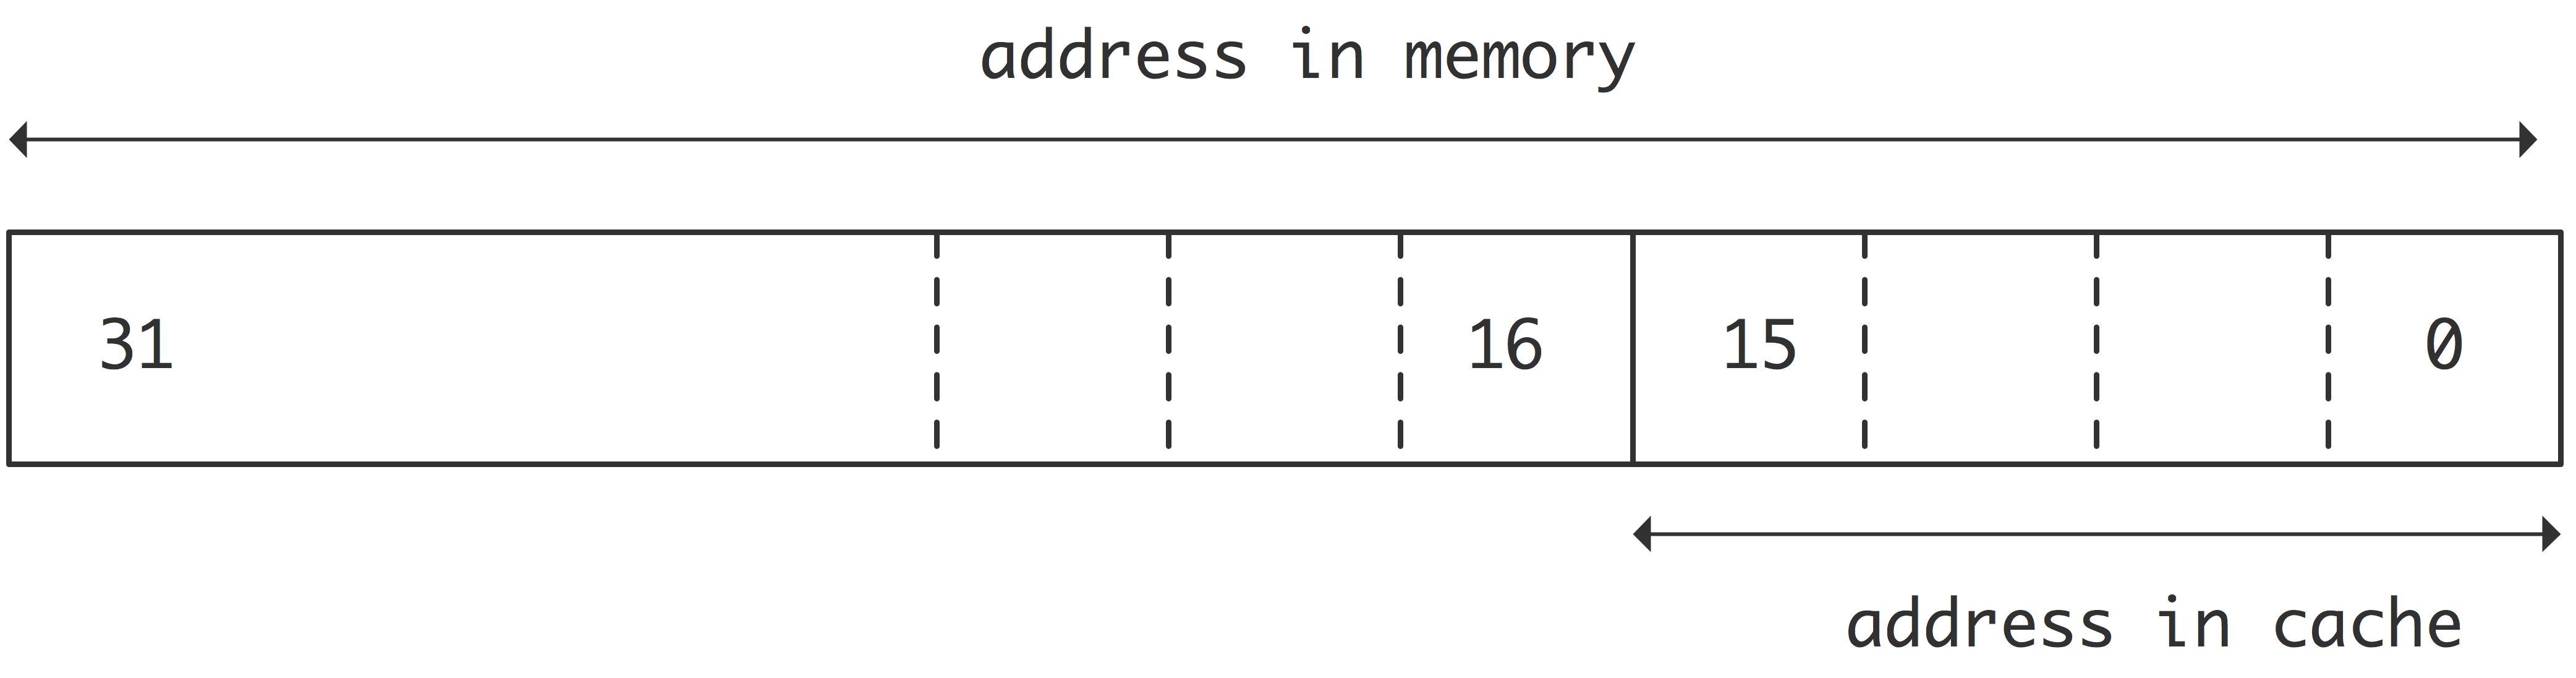
\includegraphics[scale=.1]{directmap}
  \caption{Direct mapping of 32-bit addresses into a 64K cache}
  \label{fig:directmap}
\end{figure}
and uses these as the address of the data item in cache; see figure~\ref{fig:directmap}.

Direct mapping is very efficient because of its address calculations
can be performed very quickly, leading to low latency, but it
has a problem in practical applications. If two items are addressed
that are separated by 8K words, they will be mapped to the same cache
location, which will make certain calculations inefficient. Example:
\begin{verbatim}
double A[3][8192];
for (i=0; i<512; i++)
  a[2][i] = ( a[0][i]+a[1][i] )/2.;
\end{verbatim}
or in Fortran:
\begin{verbatim}
real*8 A(8192,3);
do i=1,512
  a(i,3) = ( a(i,1)+a(i,2) )/2
end do
\end{verbatim}
Here, the locations of \texttt{a[0][i]}, \texttt{a[1][i]}, and
\texttt{a[2][i]} (or \texttt{a(i,1),a(i,2),a(i,3)})
are 8K from each other for every~\n{i}, so the last
16 bits of their addresses will be the same, and hence they will
be mapped to the same location in cache. The execution of the loop will now
go as follows:
\begin{itemize}
\item The data at \texttt{a[0][0]} is brought into cache and
  register. This engenders a certain amount of latency. Together with
  this element, a whole cache line is transferred.
\item The data at \texttt{a[1][0]} is brought into cache (and
  register, as we will not remark anymore from now on), together
  with its whole cache line, at cost of some latency. Since this cache
  line is mapped to the same location as the first, the first cache
  line is overwritten.
\item In order to write the output, the cache line containing
  \texttt{a[2][0]} is brought into memory. This is again mapped to the
  same location, causing flushing of the cache line just loaded
  for~\texttt{a[1][0]}.
\item In the next iteration, \texttt{a[0][1]} is needed, which is
  on the same cache line as \texttt{a[0][0]}. However, this cache line
  has been flushed, so it needs to be brought in anew from main memory
  or a deeper cache level. In doing so, it overwrites the cache line
  that holds \texttt{a[2][0]}.
\item A similar story hold for \texttt{a[1][1]}: it is on the cache
  line of \text{a[1][0]}, which unfortunately has been overwritten in
  the previous step.
\end{itemize}
If a cache line holds four words, we see that each four iterations of
the loop involve eight transfers of elements of~\texttt{a}, where two
would have sufficed, if it were not for the cache conflicts.

\begin{exercise}
%  (Section \ref{sec:directmap})
  In the example of direct mapped caches, mapping from memory to cache
  was done by using the final 16 bits of a 32 bit memory address as
  cache address. Show that the problems in this example go away if the
  mapping is done by using the first (`most significant') 16 bits as
  the cache address. Why is this not a good solution in general?
\end{exercise}

\Level 2 {Associative caches}
\label{sec:associative}
\index{associative|seealso{cache, associative}}.

The problem of cache conflicts, outlined in the previous section, would
be solved if any data item could go to any cache location. In that
case there would be no conflicts, other than the cache filling up, in
which case a cache replacement policy (section~\ref{sec:lru}) would
flush data to make room for the incoming item. Such a cache is called
\indexterm{fully associative}, and while it seems optimal, it is also
very costly to build, and much slower in use than a direct mapped cache.

For this reason, the most common solution is to have a
$k$-way \indextermsub{associative}{cache}, where $k$~is at least two. In
this case, a data item can go to any of $k$ cache locations. Code
would have to have a $k+1$-way conflict before data would be flushed
prematurely as in the above example. In that example, a value of $k=2$
would suffice, but in practice higher values are often encountered.
\begin{figure}[ht]
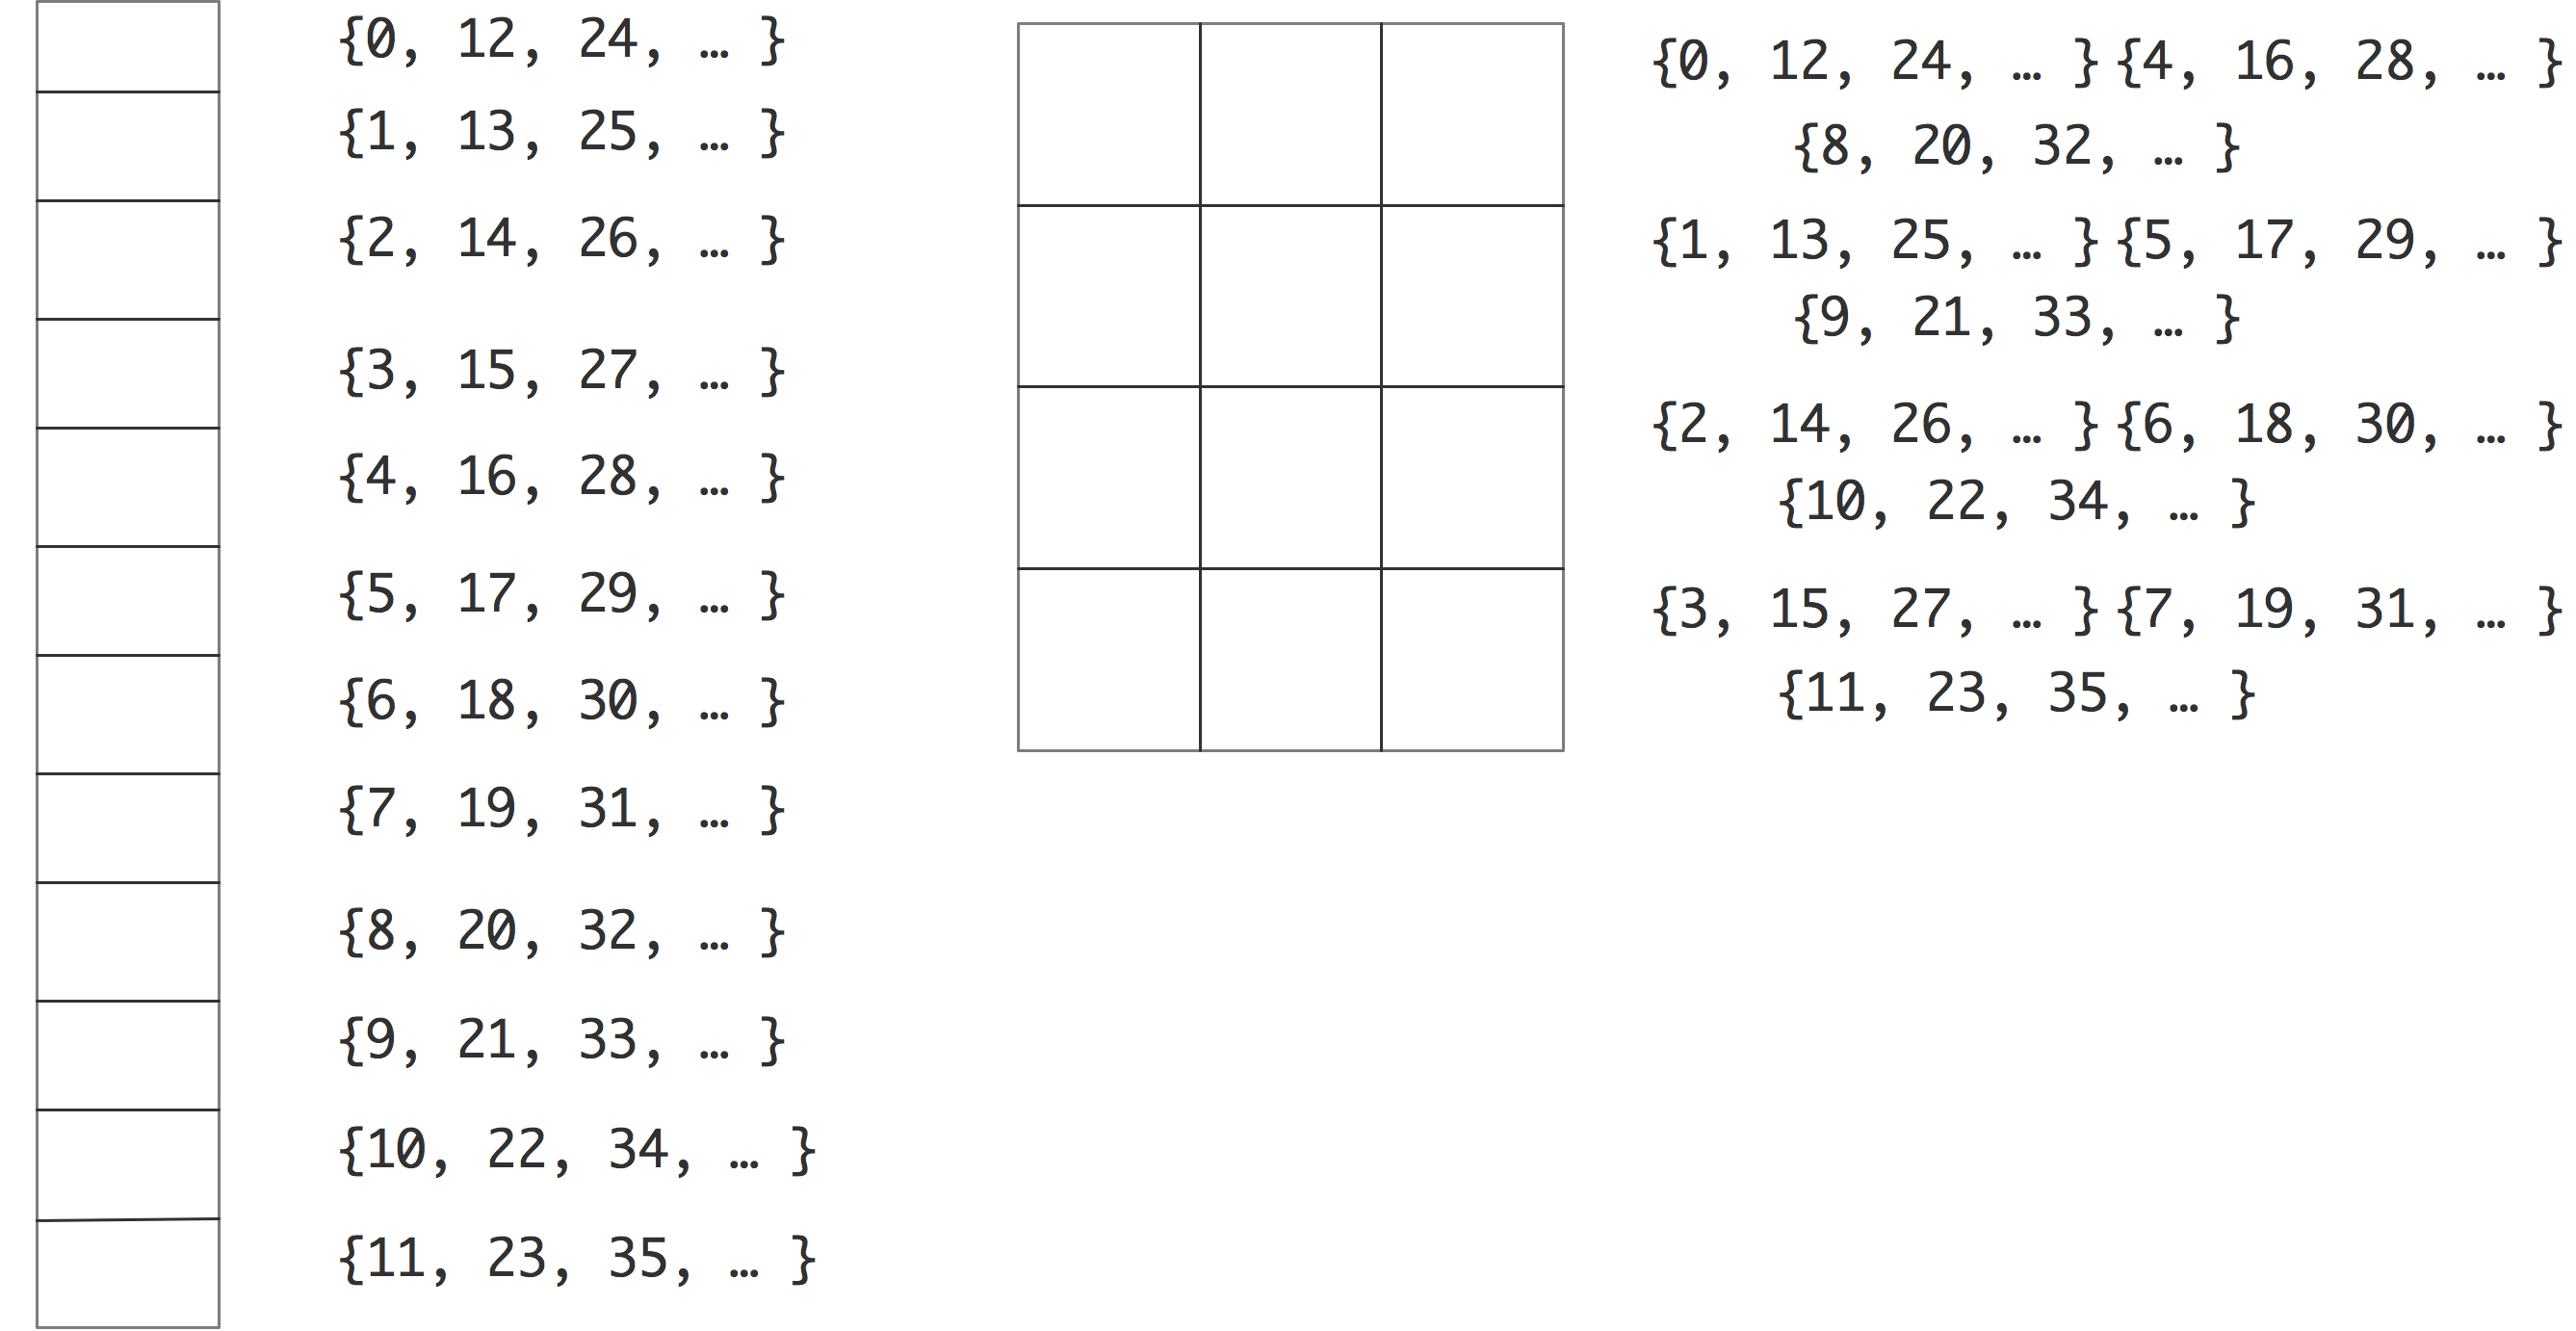
\includegraphics[scale=.12]{graphics/assoc-mapping}
\caption{Two caches of 12 elements: direct mapped (left) and 3-way associative (right)}
\label{fig:assoc-mapping}
\end{figure}
Figure~\ref{fig:assoc-mapping} illustrates the mapping of memory
addresses to cache locations for a direct mapped and a 3-way associative
cache. Both caches has 12 elements, but addressed diferently.
The direct mapped cache (left)
will have a conflict between memory address 0~and~12, but
in the 3-way associative cache these two addresses can be mapped
to any of three elements.

As a practical example, the
\indextermbus{Intel}{Woodcrest} processor has
an L1 cache of 32K bytes that is 8-way set associative with a 64
  byte cache line size, and
an L2 cache of 4M bytes that is 8-way set associative with a 64
  byte cache line size.
On the other hand, the \indextermbus{AMD}{Barcelona} chip
has 2-way associativity for the L1 cache, and 8-way for
the~L2. A~higher associativity (`way-ness') is obviously desirable,
but makes a processor slower, since determining whether an address is
already in cache becomes more complicated. For this reason, the
associativity of the L1~cache, where speed is of the greatest
importance, is typically lower than of the L2.

\begin{exercise}
  Write a small cache simulator in your favourite language. Assume a
  $k$-way associative cache of 32 entries and an architecture with 16
  bit addresses. Run the following
  experiment for $k=1,2,4,\ldots$:
  \begin{enumerate}
  \item Let $k$ be the associativity of the simulated cache.
  \item Write the translation from 16 bit memory addresses to $32/k$ 
    cache addresses.
  \item\label{step:random} Generate 32 random machine addresses, and
    simulate storing them in cache.
  \end{enumerate}
  Since the cache has 32 entries, optimally the 32 addresses can all
  be stored in cache. The chance of this actually happening is small,
  and often the data of one address will be evicted from the cache
  (meaning that it is overwritten) when another address conflicts with
  it. Record how many addresses, out of~32, are actually stored in the
  cache at the end of the simulation. Do step~\ref{step:random} 100
  times, and plot the results; give median and average value, and the
  standard deviation. Observe that increasing the associativity
  improves the number of addresses stored. What is the limit
  behaviour? (For bonus points, do a formal statistical analysis.)
\end{exercise}

\index{cache|)}

\Level 1 {Prefetch streams}
\label{sec:prefetch}

In the traditional von Neumann model (section~\ref{sec:vonneuman}),
each instruction contains the location of its operands, so a CPU
implementing this model would make a separate request for each new
operand. In practice, often subsequent data items are adjacent or
regularly spaced in memory. The memory system can try to detect such
data patterns by looking at cache miss points,
and request a \indexterm{prefetch data stream}
\begin{figure}
  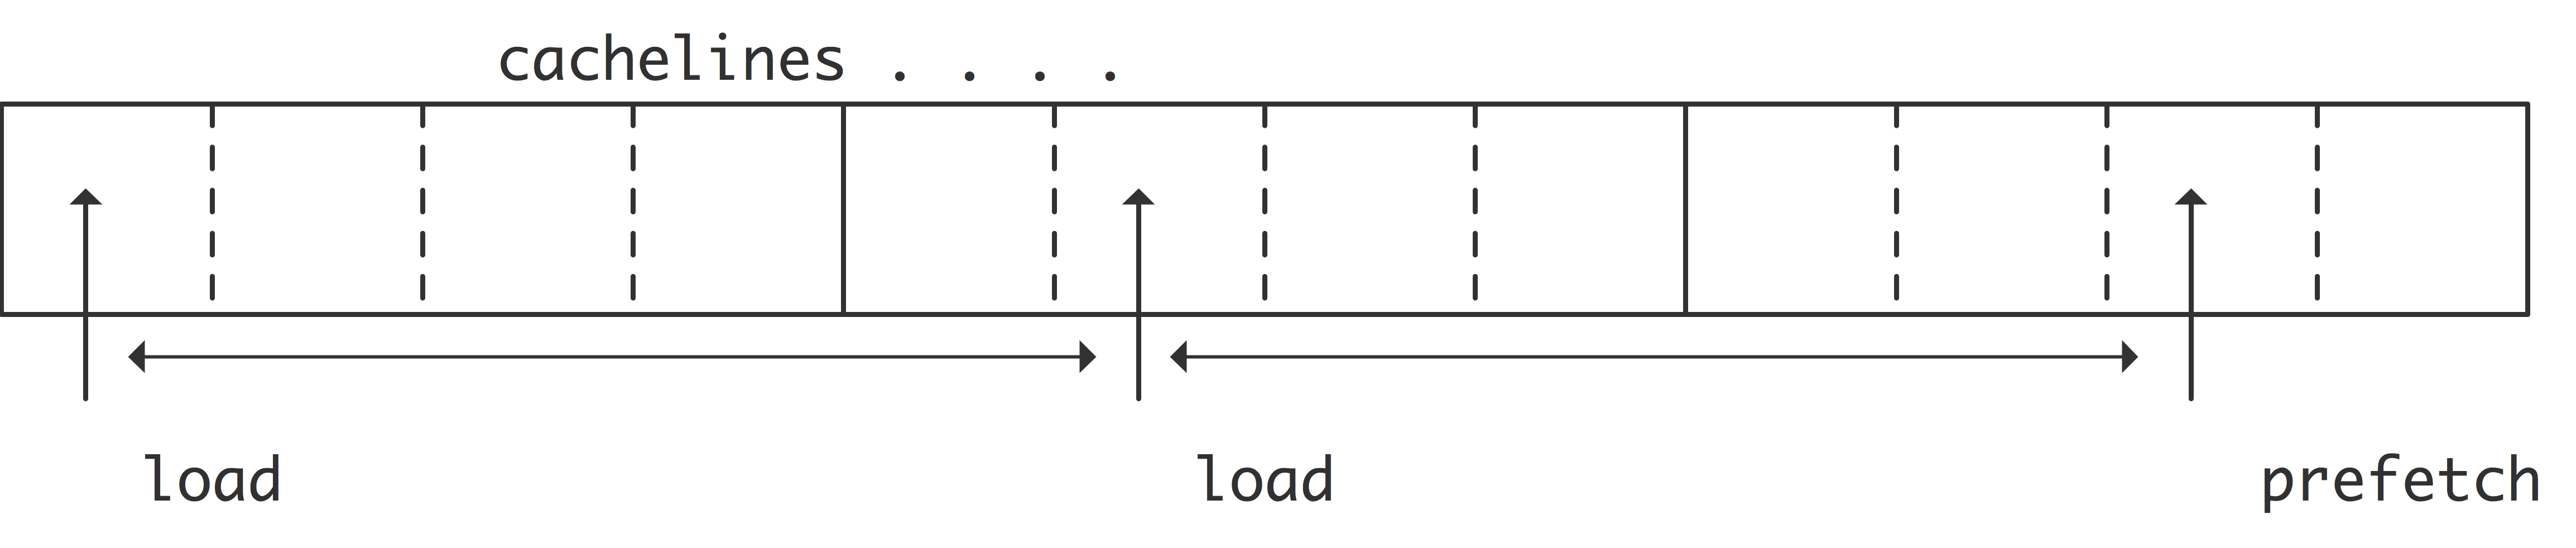
\includegraphics[scale=.09]{prefetch}
  \caption{Prefetch stream generated by equally spaced requests}
  \label{fig:prefetch}
\end{figure}
(figure~\ref{fig:prefetch}).

In its simplest form, the CPU will detect that consecutive loads come
from two consecutive cache lines, and automatically issue a request
for the next following cache line. This process can be repeated or
extended if the code makes an actual request for that third cache
line. Since these cache lines are now brought from memory well before
they are needed, prefetch has the possibility of eliminating the
latency for all but the first couple of data items.

The concept of \indextermbus{cache}{miss} now needs to be revisited a
little. From a performance point of view we are only interested in
\indexterm{stall}s on cache misses, that is, the case where the
computation has to wait for the data to be brought in. Data that is
not in cache, but can be brought in while other instructions are still
being processed, is not a problem. If an `L1 miss' is understood to be
only a `stall on miss', then the term `L1 cache refill' is used to
describe all cacheline loads, whether the processor is stalling on
them or not.

Since prefetch is controlled by the hardware, it is also described as
\indexterm{hardware prefetch}.  Prefetch streams can sometimes be
controlled from software, though often it takes assembly code,
for instance \indextermsub{inline}{assembly} instructions in your C~code,
to do so. On the \indextermbus{IBM}{BlueGene Q} prefetch can be
activated by program directives.

\Level 1 {Concurrency and memory transfer}

In the discussion about the memory hierarchy we made the point that
memory is slower than the processor. As if that is not bad enough, it
is not even trivial to exploit all the bandwidth that memory
offers. In other words, if you don't program carefully you will get
even less performance than you would expect based on the available
bandwidth. Let's analyze this.

The memory system typically has a bandwidth of more than one floating
point number per cycle, so you need to issue that many requests per
cycle to utilize the available bandwidth. This would be true even with
zero latency; since there is latency, it takes a while for data to
make it from memory and be processed. Consequently, any data requested
based on computations on the first data has to be requested with a
delay at least equal the memory latency.

For full utilization of the bandwidth,
at all times a volume of data equal to the bandwidth times
the latency has to be in flight. Since these data have to be
independent, we get a statement of \indexterm{Little's
  law}~\cite{Little:law}:
\[ \mathrm{Concurrency}=\mathrm{Bandwidth}\times \mathrm{Latency}. \]
\begin{figure}[ht]
  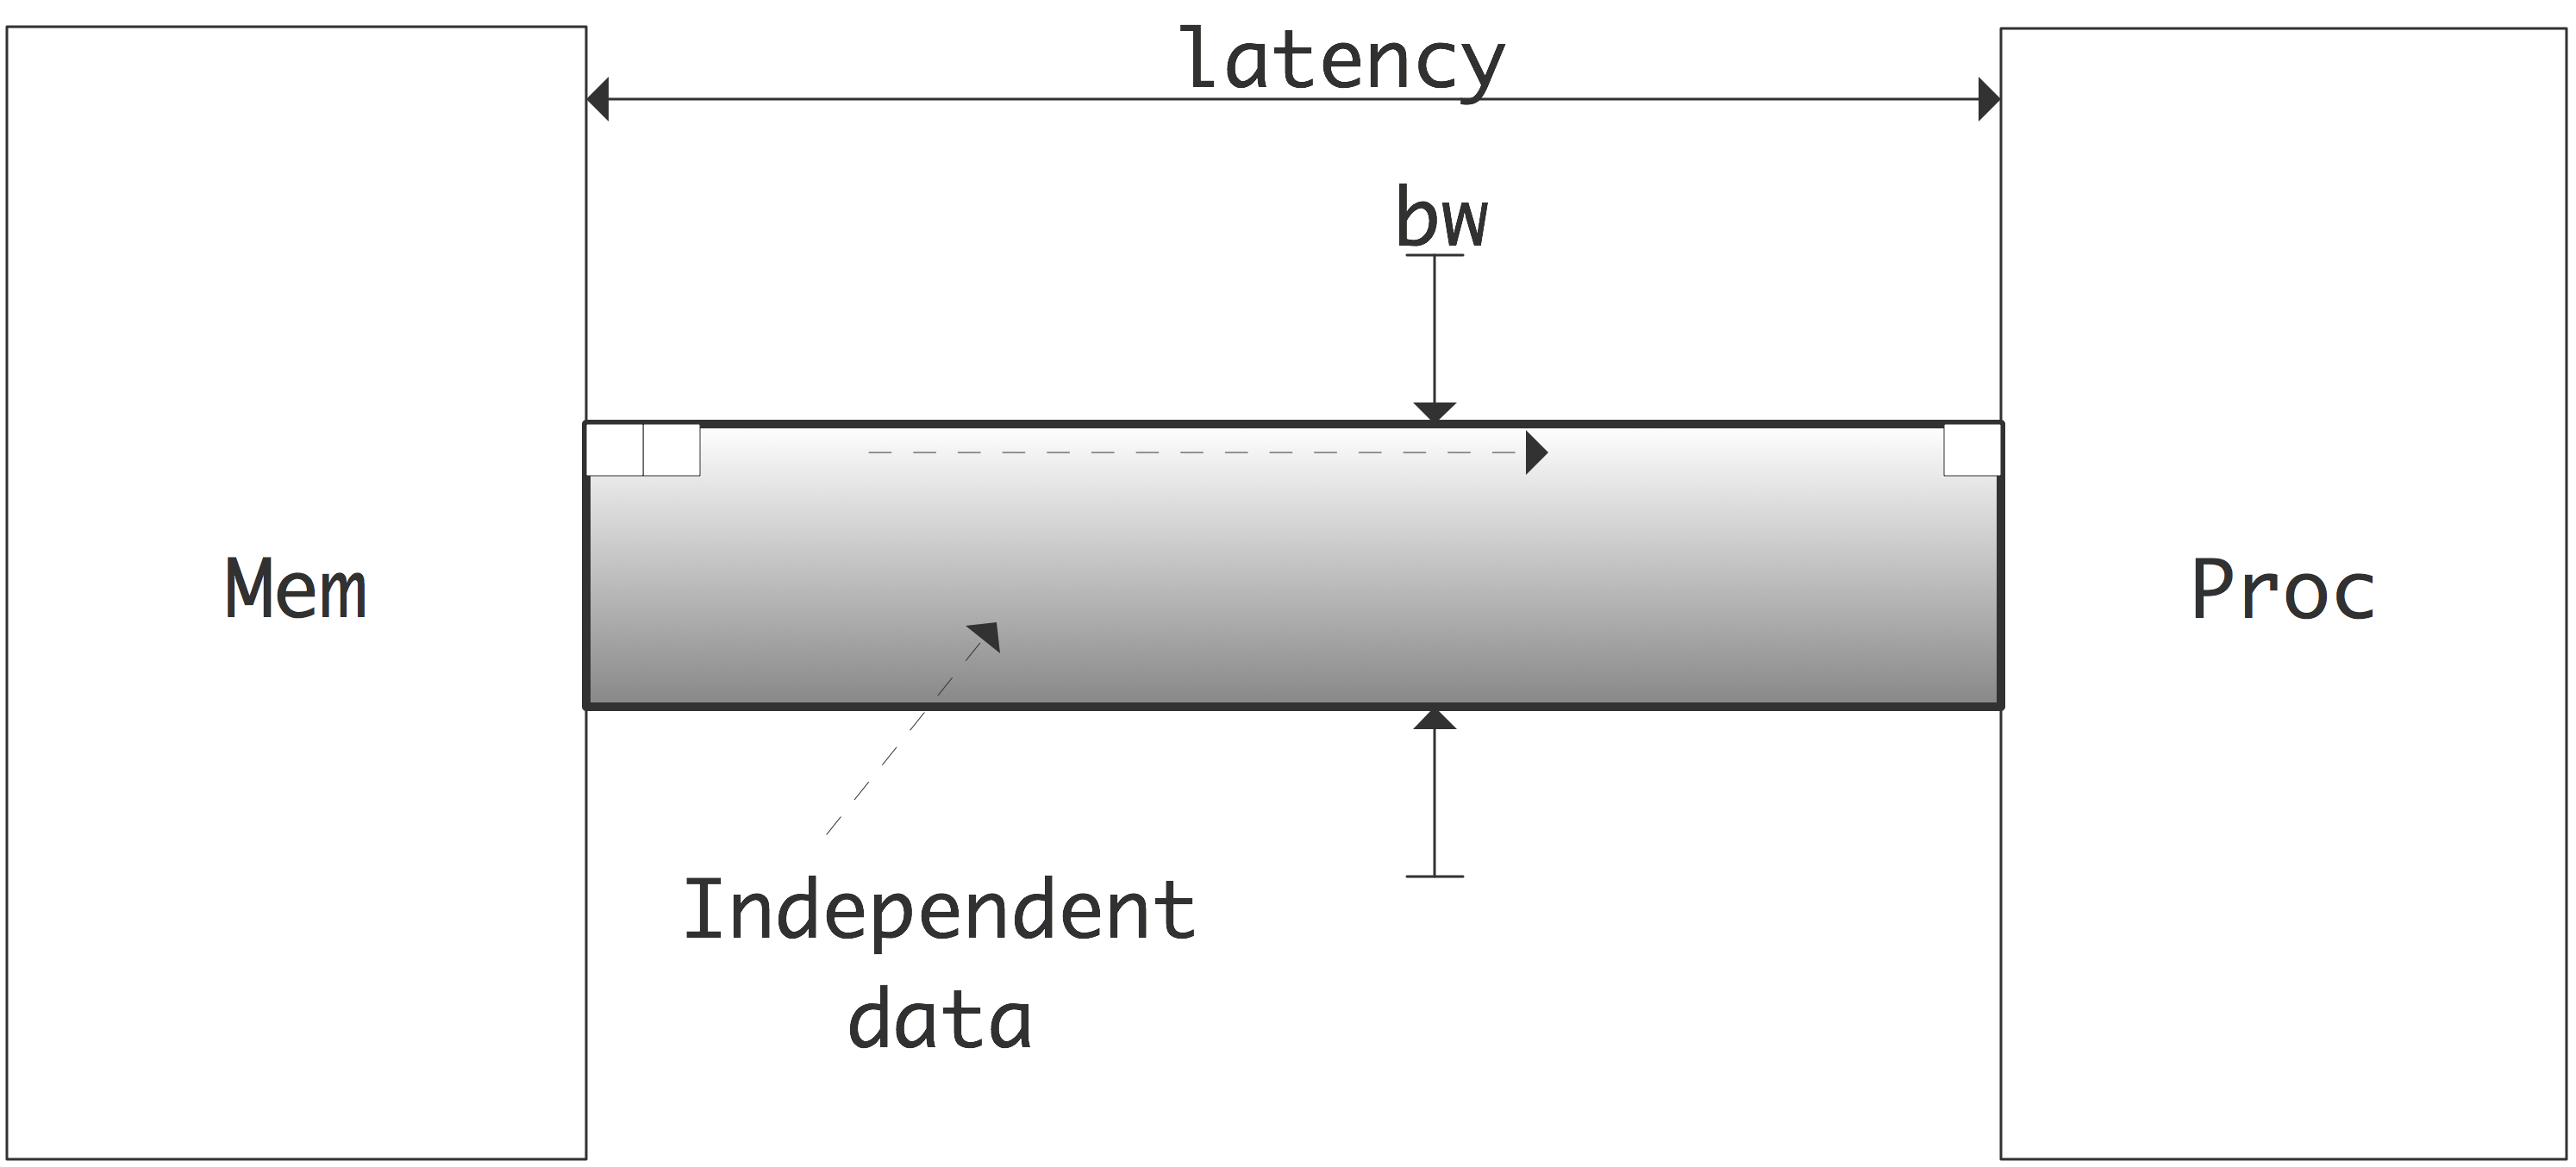
\includegraphics[scale=.13]{graphics/little}
  \caption{Illustration of Little's Law that states how much
    independent data needs to be in flight}
  \label{fig:little}
\end{figure}
This is illustrated in figure~\ref{fig:little}. The problem with
maintaining this concurrency is not that a program does not have it;
rather, the program is to get the compiler and runtime system
recognize it. For instance, if a loop traverses a long array, the
compiler will not issue a large number of memory requests. The
prefetch mechanism (section~\ref{sec:prefetch}) will issue some memory
requests ahead of time, but typically not enough. Thus, in order to
use the available bandwidth, multiple streams of data need to be under
way simultaneously. Therefore, we can also phrase Little's law as
\[ \mathrm{Effective\ throughput}=\mathrm{Expressed\ concurrency} / \mathrm{Latency}. \]

\Level 1 {Memory banks}
\label{sec:banks}

Above, we discussed issues relating to bandwdith. You saw that memory,
and to a lesser extent caches, have a bandwidth that is less than what
a processor can maximally absorb. The situation is actually even worse
than the above discussion made it seem. For this reason, memory is
often divided into \indextermbus{memory}{banks} that are interleaved: with
four memory banks, words $0,4,8,\ldots$ are in bank~0, words
$1,5,9,\ldots$ are in bank~1, et cetera. 

Suppose we now access memory sequentially, then such 4-way interleaved
memory can sustain four times the bandwidth of a single memory
bank. Unfortunately,  accessing by stride~2 will halve the bandwidth,
and larger strides are even worse. In practice the number of memory
banks will be higher, so that strided memory access with small strides
will still have the full advertised bandwidth.

This concept of banks can also apply to caches. For instance, the
cache lines in the L1 cache of the \indextermbus{AMD}{Barcelona} chip
are 16 words long, divided into two interleaved banks of 8 words. This
means that sequential access to the elements of a cache line is
efficient, but strided access suffers from a deteriorated performance.


\Level 1 {TLB and virtual memory}
\label{sec:tlb}

All of a program's data may not be in memory simultaneously. This can
happen for a number of reasons:
\begin{itemize}
\item The computer serves multiple users, so the memory is not
  dedicated to any one user;
\item The computer is running multiple programs, which together need
  more than the physically available memory;
\item One single program can use more data than the available memory.
\end{itemize}
For this reason, computers use \indexterm{Virtual memory}: if more
memory is needed than is available, certain blocks of memory are
written to disc. In effect, the disc acts as an extension of the real
memory. This means that a block of data can be anywhere in memory, and
in fact, if it is \indexterm{swapped} in and out, it can be in
different locations at different times. Swapping does not act on
individual memory locations, but rather on \indextermbus{memory}{pages}:
\index{pages!memory|see{memory, pages}}
contiguous blocks of memory, from a few kilobytes to megabytes in size.
(In an earlier generation of operating systems, moving memory to disc
was a programmer's responsibility. Pages that would replace each other
were called \indexterm{overlays}.)

For this reason, we need a translation mechanism from the memory
addresses that the program uses to the actual addresses in memory, and
this translation has to be dynamic. A~program has a `logical data
space' (typically starting from address zero) of the addresses used in
the compiled code, and this needs to be translated during program
execution to actual memory addresses. For this reason, there is a
\indexterm{page table} that specifies which memory pages contain which
logical pages.

However, address translation by lookup in this table is slow, so CPUs
have a \indexac{TLB}.
The \ac{TLB} is a cache of frequently used 
Page Table Entries: it provides fast address translation for a number
of pages. If a program needs a memory
location, the \ac{TLB} is consulted to see whether this location is in fact
on a page that is remembered in the \ac{TLB}. 
If this is the case, the logical address is
translated to a physical one; this is a very fast process. The case
where the page is not remembered in the \ac{TLB} is called a
\indextermbus{TLB}{miss}, and the page lookup table is then consulted,
if necessary bringing the needed page into memory.
The \ac{TLB} is (sometimes fully) associative
(section~\ref{sec:associative}), using an LRU policy
(section~\ref{sec:lru}).

A typical \ac{TLB} has between 64 and 512 entries. If a program accesses
data sequentially, it will typically alternate between just a few
pages, and there will be no \ac{TLB} misses. On the other hand, a program
that access many random memory locations can experience a slowdown
because of such misses. 

Section~\ref{sec:coding-tlb} and appendix~\ref{sec:tlb-code} discuss
some simple code illustrating the
behaviour of the \ac{TLB}.

[There are some complications to this story. For instance, there is
  usually more than one \ac{TLB}. The first one is associated with the
  L2~cache, the second one with the~L1. In the
  \indextermbus{AMD}{Opteron}, the L1~\ac{TLB} has 48 entries, and
  is is fully (48-way) associative, while the L2~\ac{TLB} has 512
  entries, but is only 4-way associative. This means that there can
  actually be \ac{TLB} conflicts. In the discussion above, we have
  only talked about the L2 \ac{TLB}. The reason that this can be
  associated with the L2~cache, rather than with main memory, is that
  the translation from memory to L2~cache is deterministic.]

\Level 0 {Multicore architectures}
\label{sec:multicore}
\index{multicore|(textbf}

In recent years, the limits of performance have been reached for the
traditional processor chip design.
\begin{itemize}
\item Clock frequency can not be increased further, since it increases
  energy consumption, heating the chips too
  much; see section~\ref{sec:power}. 
\item It is not possible to extract more \acf{ILP}
  from codes, either because of compiler limitations, because of the
  limited amount of intrinsically available parallelism, or because
  branch prediction makes it impossible (see
  section~\ref{sec:pipelinecpu}).
\end{itemize}

One of the ways of getting a higher utilization out of a single
processor chip is then to move from a strategy of further
sophistication of the single processor, to a division of the chip into
multiple processing `cores'\footnote{Another solution is Intel\index{Intel}'s
  \indexterm{hyperthreading}, which lets a processor mix the instructions of
  several instruction streams. The benefits of this are strongly
  dependent on the individual case. However, this same mechanism is
  exploited with great success in GPUs; see
  section~\ref{sec:gpu}. For a discussion see section~\ref{sec:hyperthread}}.
The separate cores can work on unrelated
tasks, or, by introducing what is in effect data parallelism
(section~\ref{sec:simd}), collaborate on a common task at a higher
overall efficiency.

This solves the above two problems:
\begin{itemize}
\item Two cores at a lower frequency can have the same throughput as a
  single processor at a higher frequency; hence, multiple cores are
  more energy-efficient.
\item Discovered \ac{ILP} is now replaced by explicit task
  parallelism, managed by the programmer.
\end{itemize}

While the first multicore CPUs
were simply two processors on the same die, later generations
incorporated L3 or L2 caches that were shared between the two
processor cores; see figure~\ref{fig:core-caches}
\begin{figure}[ht]
  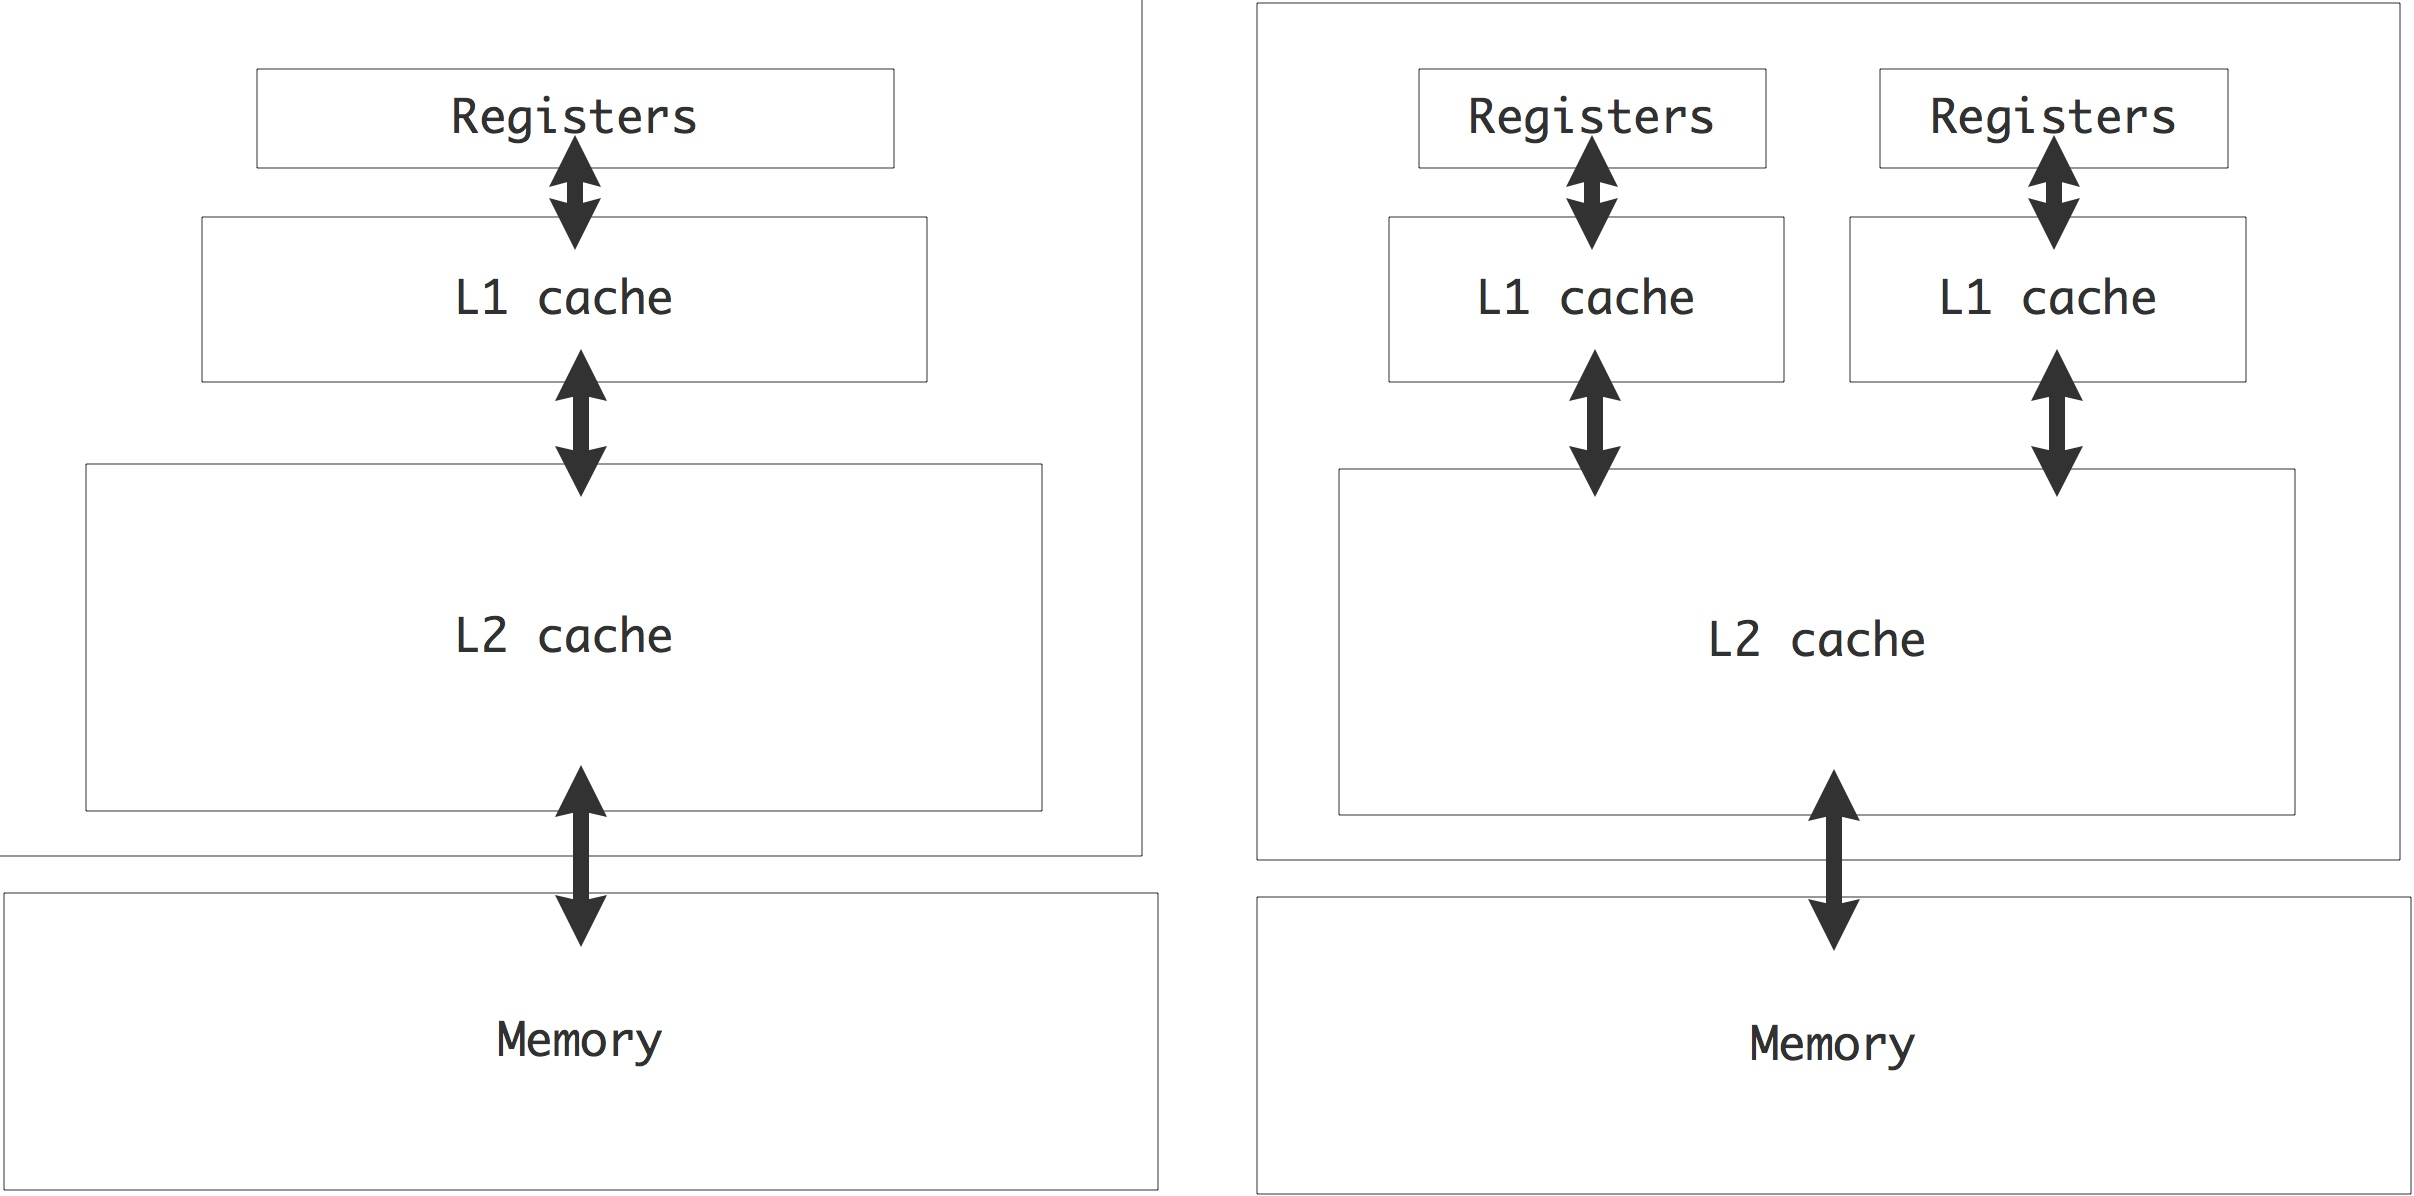
\includegraphics[scale=.18]{graphics/cache-hierarchy}
  \caption{Cache hiearchy in a single-core and dual-core chip}
  \label{fig:core-caches}
\end{figure}
This design makes it efficient for the cores to work
jointly on the same problem. 
The cores would still have their own L1 cache, and these separate
caches lead to a \indextermbus{cache}{coherence} problem; see
section~\ref{sec:coherence} below.

We note that the term `processor' is now ambiguous: it can refer to either the
chip, or the processor core on the chip. For this reason, we mostly
talk about a \indexterm{socket} for the whole chip and
\indexterm{core}\index{core!vs processor}
for the part containing one arithmetic and logic unit and
having its own registers. Currently, CPUs with 4 or 6 cores are
common,
even in laptops, and Intel and AMD are marketing 12-core chips.
The core count is
likely to go up in the future: Intel\index{Intel}
has already shown an 80-core prototype that is developed into the 48
core `Single-chip Cloud Computer', illustrated in
fig~\ref{fig:rockcreek}. This chip has a structure with 24 dual-core
`tiles' that are connected through a 2D mesh network. Only certain
tiles are connected to a memory controller, others can not reach
memory other than through the on-chip network.

\begin{figure}[ht]
  \begin{quote}
  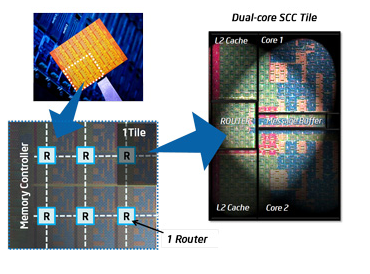
\includegraphics[scale=.5]{graphics/ScCC-1}
  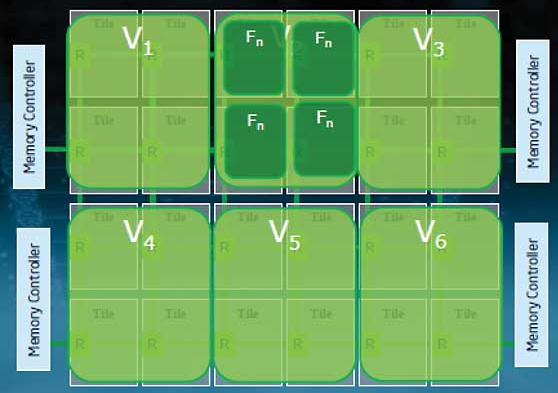
\includegraphics[scale=.4]{graphics/ScCC-2}
  \end{quote}
  \caption{Structure of the Intel Single-chip Cloud Computer chip}
  \label{fig:rockcreek}
\end{figure}

With
this mix of shared and private caches, the programming model for
multicore processors is becoming a hybrid between shared and
distributed memory:
\begin{itemize}
\item[{\it Core}] The cores have their own private L1 cache, which is a sort of
  distributed memory. The above mentioned Intel 80-core prototype has the
  cores communicating in a distributed memory fashion.
\item[{\it Socket}] On one socket, there is often a shared L2 cache, which is shared
  memory for the cores.
\item[{\it Node}] There can be multiple sockets on a single `node' or
  motherboard, accessing the same shared memory.
\item[{\it Network}] Distributed memory programming (see the next
  chapter) is needed to let nodes
  communicate.
\end{itemize}

Historically, multicore architectures have a precedent in
multiprocessor shared memory designs (section~\ref{sec:uma}) such as
the \indexterm{Sequent Symmetry} and the \indexterm{Alliant
  FX/8}. Conceptually the program model is the same, but the
technology now allows to shrink a multiprocessor board to a multicore
chip.

\Level 1 {Cache coherence}
\label{sec:coherence}
\index{cache!coherence|(}

With parallel processing, there is the potential for a conflict if more
than one processor has a copy of the same data item. The problem of
ensuring that all cached data are an accurate copy of main memory, is
referred to as \emph{cache coherence}: if one processor alters
its copy, the other copy needs to be updated.

In distributed memory architectures, a dataset is usually partitioned
disjointly over the processors, so conflicting copies of data can only
arise with knowledge of the user, and it is up to the user to
deal with the problem. The case of shared memory is more subtle: since
processes access the same main memory, it would seem that conflicts
are in fact impossible. However, processor typically have some private
cache, which contains copies of data from memory, so conflicting
copies can occur.  This situation arises in particular in multicore
designs.

Suppose that two cores have a copy of the same data item in their
(private) L1 cache, and one modifies its copy. Now the other has
cached data that is no longer an accurate copy of its counterpart: the
processor will \emph{invalidate}\index{cacheline!invalidation} that
copy of the item, and in fact its whole cacheline. When the process
needs access to the item again, it needs to reload that cacheline.
The alternative is for any core that alters data to send that
cacheline to the other cores. This strategy probably has a higher overhead,
since other cores are not likely to have a copy of a cacheline.

This process of updating or invalidating cachelines
is known as \emph{maintaining cache coherence}, and it is done on
a very low level of the processor, with no programmer involvement
needed. (This makes updating memory locations an \indexterm{atomic
  operation}; more about this in section~\ref{sec:shared-lock}.)
However, it will slow down the computation, and it wastes bandwidth to
the core that could otherwise be used for loading or storing operands.

The state of a cache line with respect to a data item in main memory
is usually described as one of the following:
\begin{itemize}
\item[Scratch:] the cache line does not contain a copy of the item;
\item[Valid:] the cache line is a correct copy of data in main memory;
\item[Reserved:] the cache line is the \emph{only} copy of that piece
  of data;
\item[Dirty:] the cache line has been modified, but not yet written
  back to main memory;
\item [Invalid:] the data on the cache line is also present on other
  processors (it is not \emph{reserved}), and another process has
  modified its copy of the data.
\end{itemize}

A simpler variant of this is the \acf{MSI} coherence protocol, where a
cache line can be in the following states on a given core:
\begin{itemize}
\item [Modified:] the cacheline has been modified, and needs to be
  written to the backing store. This writing can be done when the line
  is \indexterm{evicted}, or it is done immediately, depending on the
  write-back policy.
\item [Shared:] the line is present in at least one cache and is unmodified.
\item [Invalid:] the line is not present in the current cache, or it
  is present but a copy in another cache has been modified.
\end{itemize}

These states control the movement of cachelines between memory and the
caches. For instance, suppose a core does a read to a cacheline that
is invalid on that core. It can then load it from memory or get it
from another cache, which may be faster. (Finding whether a line exists
(in state M or~S) on another cache is called \indexterm{snooping}; an alternative
is to maintain cache directories.) If
the line is Shared, it can now simply be copied; if it is in state~M in
the other cache, that core first needs to write it back to memory.

\begin{exercise}
  Consider two processors, a data item $x$ in memory, and cachelines
  $x_1$,$x_2$ in the private caches of the two processors to which $x$
  is mapped. Describe the transitions between the states of $x_1$ and
  $x_2$ under reads and writes of~$x$ on the two processors. Also
  indicate which actions cause memory bandwidth to be used. (This list
  of transitions is a \indexacf{FSA}; see section~\ref{app:fsa}.)
\end{exercise}

Variants of the \ac{MSI} protocal add an `Exclusive' or `Owned' state
for increased efficiency.

\Level 2 {Snooping}

The \indexterm{snooping} mechanism can also be used as follows: if a core
`listens in' on all bus traffic, it can invalidate or update its own cacheline 
copies when another core modifies its copy. Invalidating is cheaper than updating
since it is a bit operation, while updating involves copying the whole cacheline.

\begin{exercise}
  When would updating pay off? Write a simple cache simulator to evaluate this question.
\end{exercise}

\Level 2 {False sharing}
\label{sec:falseshare}

The cache coherence problem can even appear if the cores access
different items. For instance, a declaration
\begin{verbatim}
  double x,y;
\end{verbatim}
will likely allocate \n{x} and~\n{y} next to each other in memory, so
there is a high chance they fall on the same cacheline. Now if one
core updates~\n{x} and the other~\n{y}, this cacheline will
continuously be moved between the cores. This is called
\indexterm{false sharing|underline}.
The most common case of false sharing happens when
threads update consecutive locations of an array:
\begin{verbatim}
local_results[thread_num] = ....
\end{verbatim}

\index{cache!coherence|)}

\Level 1 {Computations on multicore chips}

Multicore chips offer a form of shared memory parallelism and can be
programmed as such, for instance using OpenMP
(section~\ref{sec:openmp}). We will go discuss in some detail the
scheduling of linear algebra operations on multicore chips;
section~\ref{sec:multicore-block}.

\index{multicore|)}

\Level 0 {Locality and data reuse}

By now it should be clear that there is more to the execution of an
algorithm than counting the operations: the data transfer involved is
important, and can in fact dominate the cost. Since we have caches and
registers, the amount of data transfer can be minimized by programming
in such a way that data stays as close to the processor as
possible. Partly this is a matter of programming cleverly, but we can
also look at the theoretical question: does the algorithm allow for it
to begin with.

It turns out that in scientific computing there is often data often
interacts mostly with data that is close by in some sense, which will
lead to data locality; section~\ref{sec:locality}. Often such locality
derives from the nature of the application, as in the case of the \acp{PDE} you
will see in chapter~\ref{ch:odepde}. In other cases such as molecular
dynamics (chapter~\ref{app:md}) there is no such intrinsic locality
because all particles interact with all others,
and considerable programming cleverness is needed to get high performance.

\Level 1 {Data reuse and arithmetic intensity}
\label{sec:reuse}
\label{sec:gemm}
\label{sec:intensity}

In the previous sections you learned that processor design is somewhat unbalanced:
loading data is slower than executing the actual operations.
This imbalance is large for main memory and less for the various cache levels.
Thus we are motivated to keep data in cache and 
keep the amount of \indexterm{data reuse}  as high as possible.

Of course, we need to determine first if the computation allows for data to be
reused.
For this we define the \indextermbus{arithmetic}{intensity} 
of an algorithm as follows:
\begin{quote}
  If $n$ is the number of data items that an algorithm operates on, and
  $f(n)$ the number of operations it takes, then the arithmetic intensity is
  $f(n)/n$.
\end{quote}
(We can measure data items in either floating point numbers or bytes.
The latter possibility makes it easier to relate arithmetic intensity
to hardware specifications of a processor.)

Arithmetic intensity is also related to \indextermbus{latency}{hiding}:
the concept that you can mitigate the negative performance impact
of data loading
behind computational activity going on.
%
For this to work, you need more computations than data loads to make
this hiding effective. And that is the very definition of
computational intensity: a high ratio of operations per
byte/word/number loaded.

\Level 2 {Examples}

Consider for example the vector addition 
\[ \forall_i\colon x_i\leftarrow x_i+y_i.
\]
This involves three memory accesses (two loads and one store) 
and one operation per iteration,
giving a arithmetic intensity of~$1/3$. The \indexterm{axpy} (for
`\emph{a}~times \emph{x} plus~\emph{y}) operation 
\[ \forall_i\colon x_i\leftarrow x_i+a\cdot y_i
\]
has
two operations, but the same number of memory access since the
one-time load of~$a$ is amortized. It is therefore more efficient
than the simple addition, with a reuse of~$2/3$.

The inner product calculation 
\[ \forall_i\colon s\leftarrow s+x_i\cdot y_i
\]
is similar in structure to the axpy operation, involving one
multiplication and addition per iteration, on two vectors and one
scalar. However, now there are only two load operations, since $s$~can
be kept in register and only written back to memory at the end of the
loop. The reuse here is~$1$.

%\Level 1 {Matrix-matrix product}

Next, consider the \emph{matrix-matrix product}\index{matrix-matrix product!reuse in}:
\[ \forall_{i,j}\colon c_{ij} = \sum_k a_{ik}b_{kj}. \] This involves
$3n^2$ data items and $2n^3$ operations, which is of a
higher order. The arithmetic intensity is~$O(n)$, meaning that every data item
will be used $O(n)$ times.  This has the implication that, with
suitable programming, this operation has the potential of overcoming
the bandwidth/clock speed gap by keeping data in fast cache memory.

\begin{exercise}
  The matrix-matrix product, considered \emph{as operation}, clearly
  has data reuse by the above definition. Argue that this reuse is not
  trivially attained by a simple implementation. What determines
  whether the naive implementation has  reuse of data that is in cache?
\end{exercise}

[In this discussion we were only concerned with the number of
  operations of a given \emph{implementation}, not the mathematical
  \emph{operation}. For instance, there are ways of performing the
  matrix-matrix multiplication and Gaussian elimination algorithms in
  fewer than $O(n^3)$
  operations~\cite{St:gaussnotoptimal,Pa:combinations}. However, this
  requires a different implementation, which has its own analysis in
  terms of memory access and reuse.]

The matrix-matrix product is the heart of the \indextermbus{LINPACK}
{benchmark}~\cite{Dongarra1987LinpackBenchmark}; see
section~\ref{sec:top500}. Using this as the solve measure of
\indexterm{benchmarking} a computer may give an optimistic view of its
performance: the matrix-matrix product is an operation
that has considerable data reuse, so it is relatively insensitive to
memory bandwidth and, for parallel computers, properties of the
network. Typically, computers will attain 60--90\% of their
\indexterm{peak performance} on the Linpack benchmark. Other benchmark
may give considerably lower figures.

\Level 2 {The roofline model}
\label{sec:roofline}
\index{roofline model|(}

There is an elegant way of talking about how arithemtic intensity,
which is a statement about the ideal algorithm, not its implementation,
interacts with hardware parameters and the actual implementation
to determine performance.
This is known as the \emph{roofline model}~\cite{Williams:2009:roofline},
and it expresses the basic fact that performance is bounded by two factors,
illustrated in the left graph of figure~\ref{fig:roofline}.
\begin{figure}[p]

  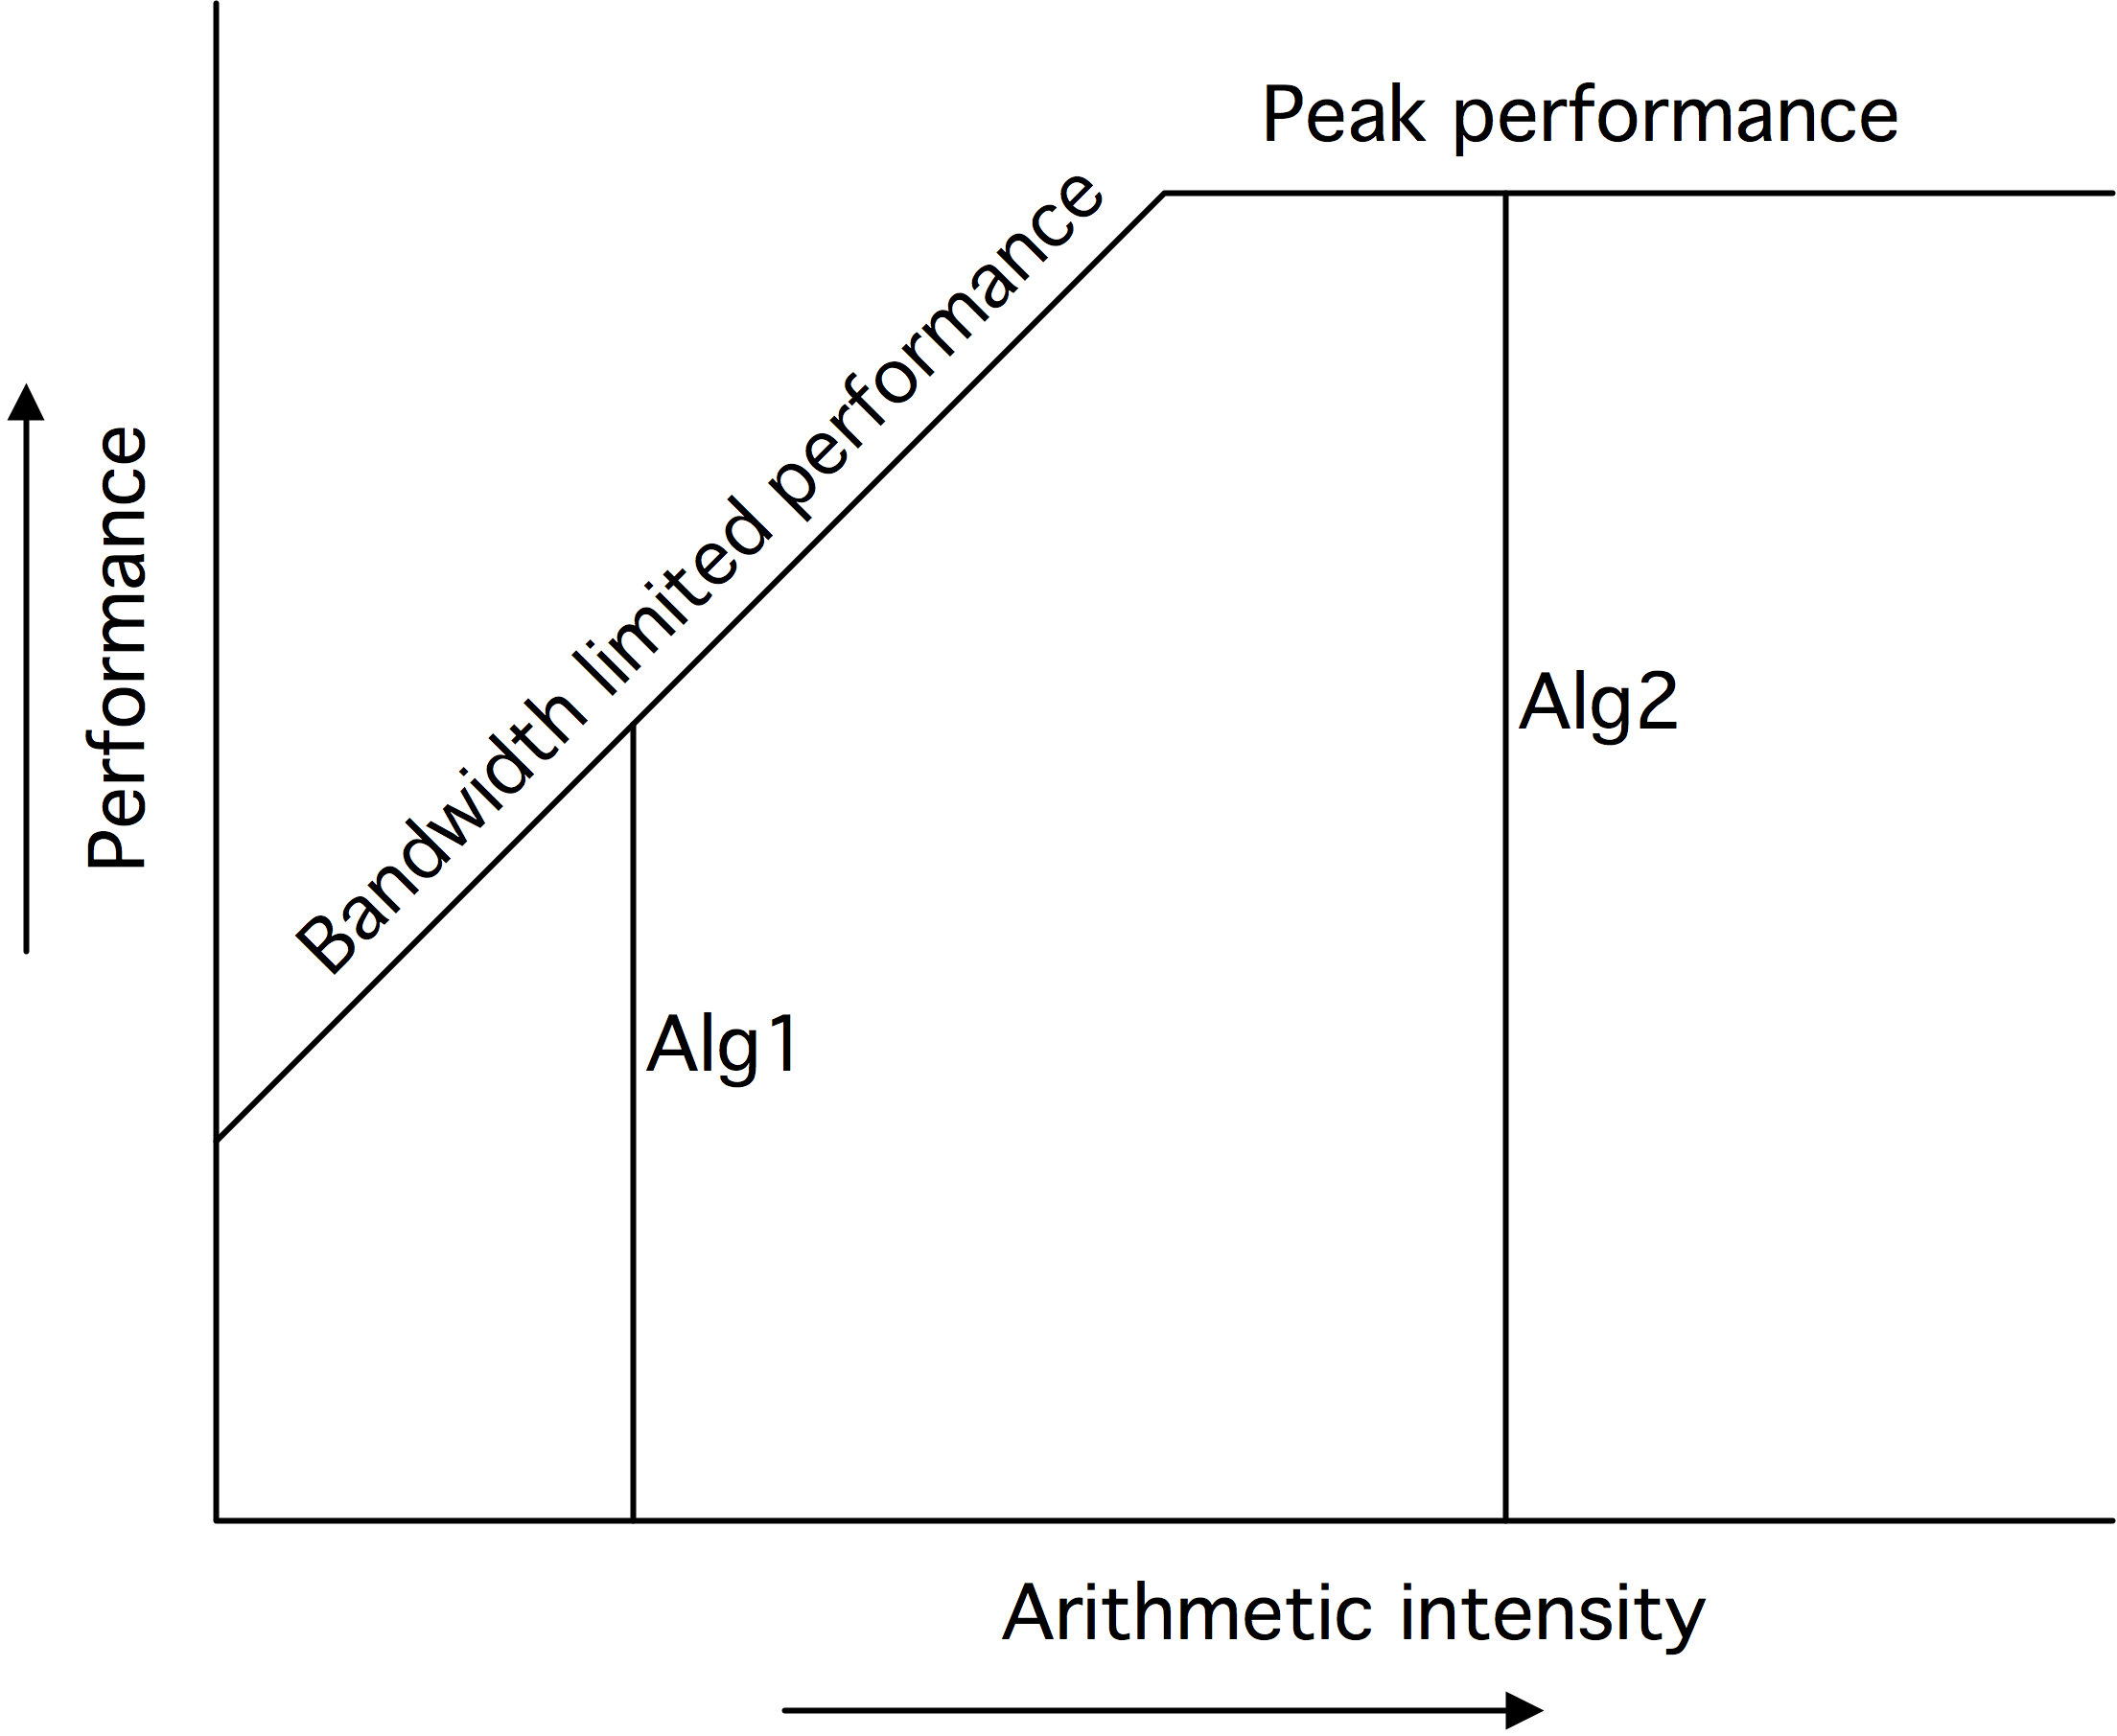
\includegraphics[scale=.1]{graphics/roofline1}
  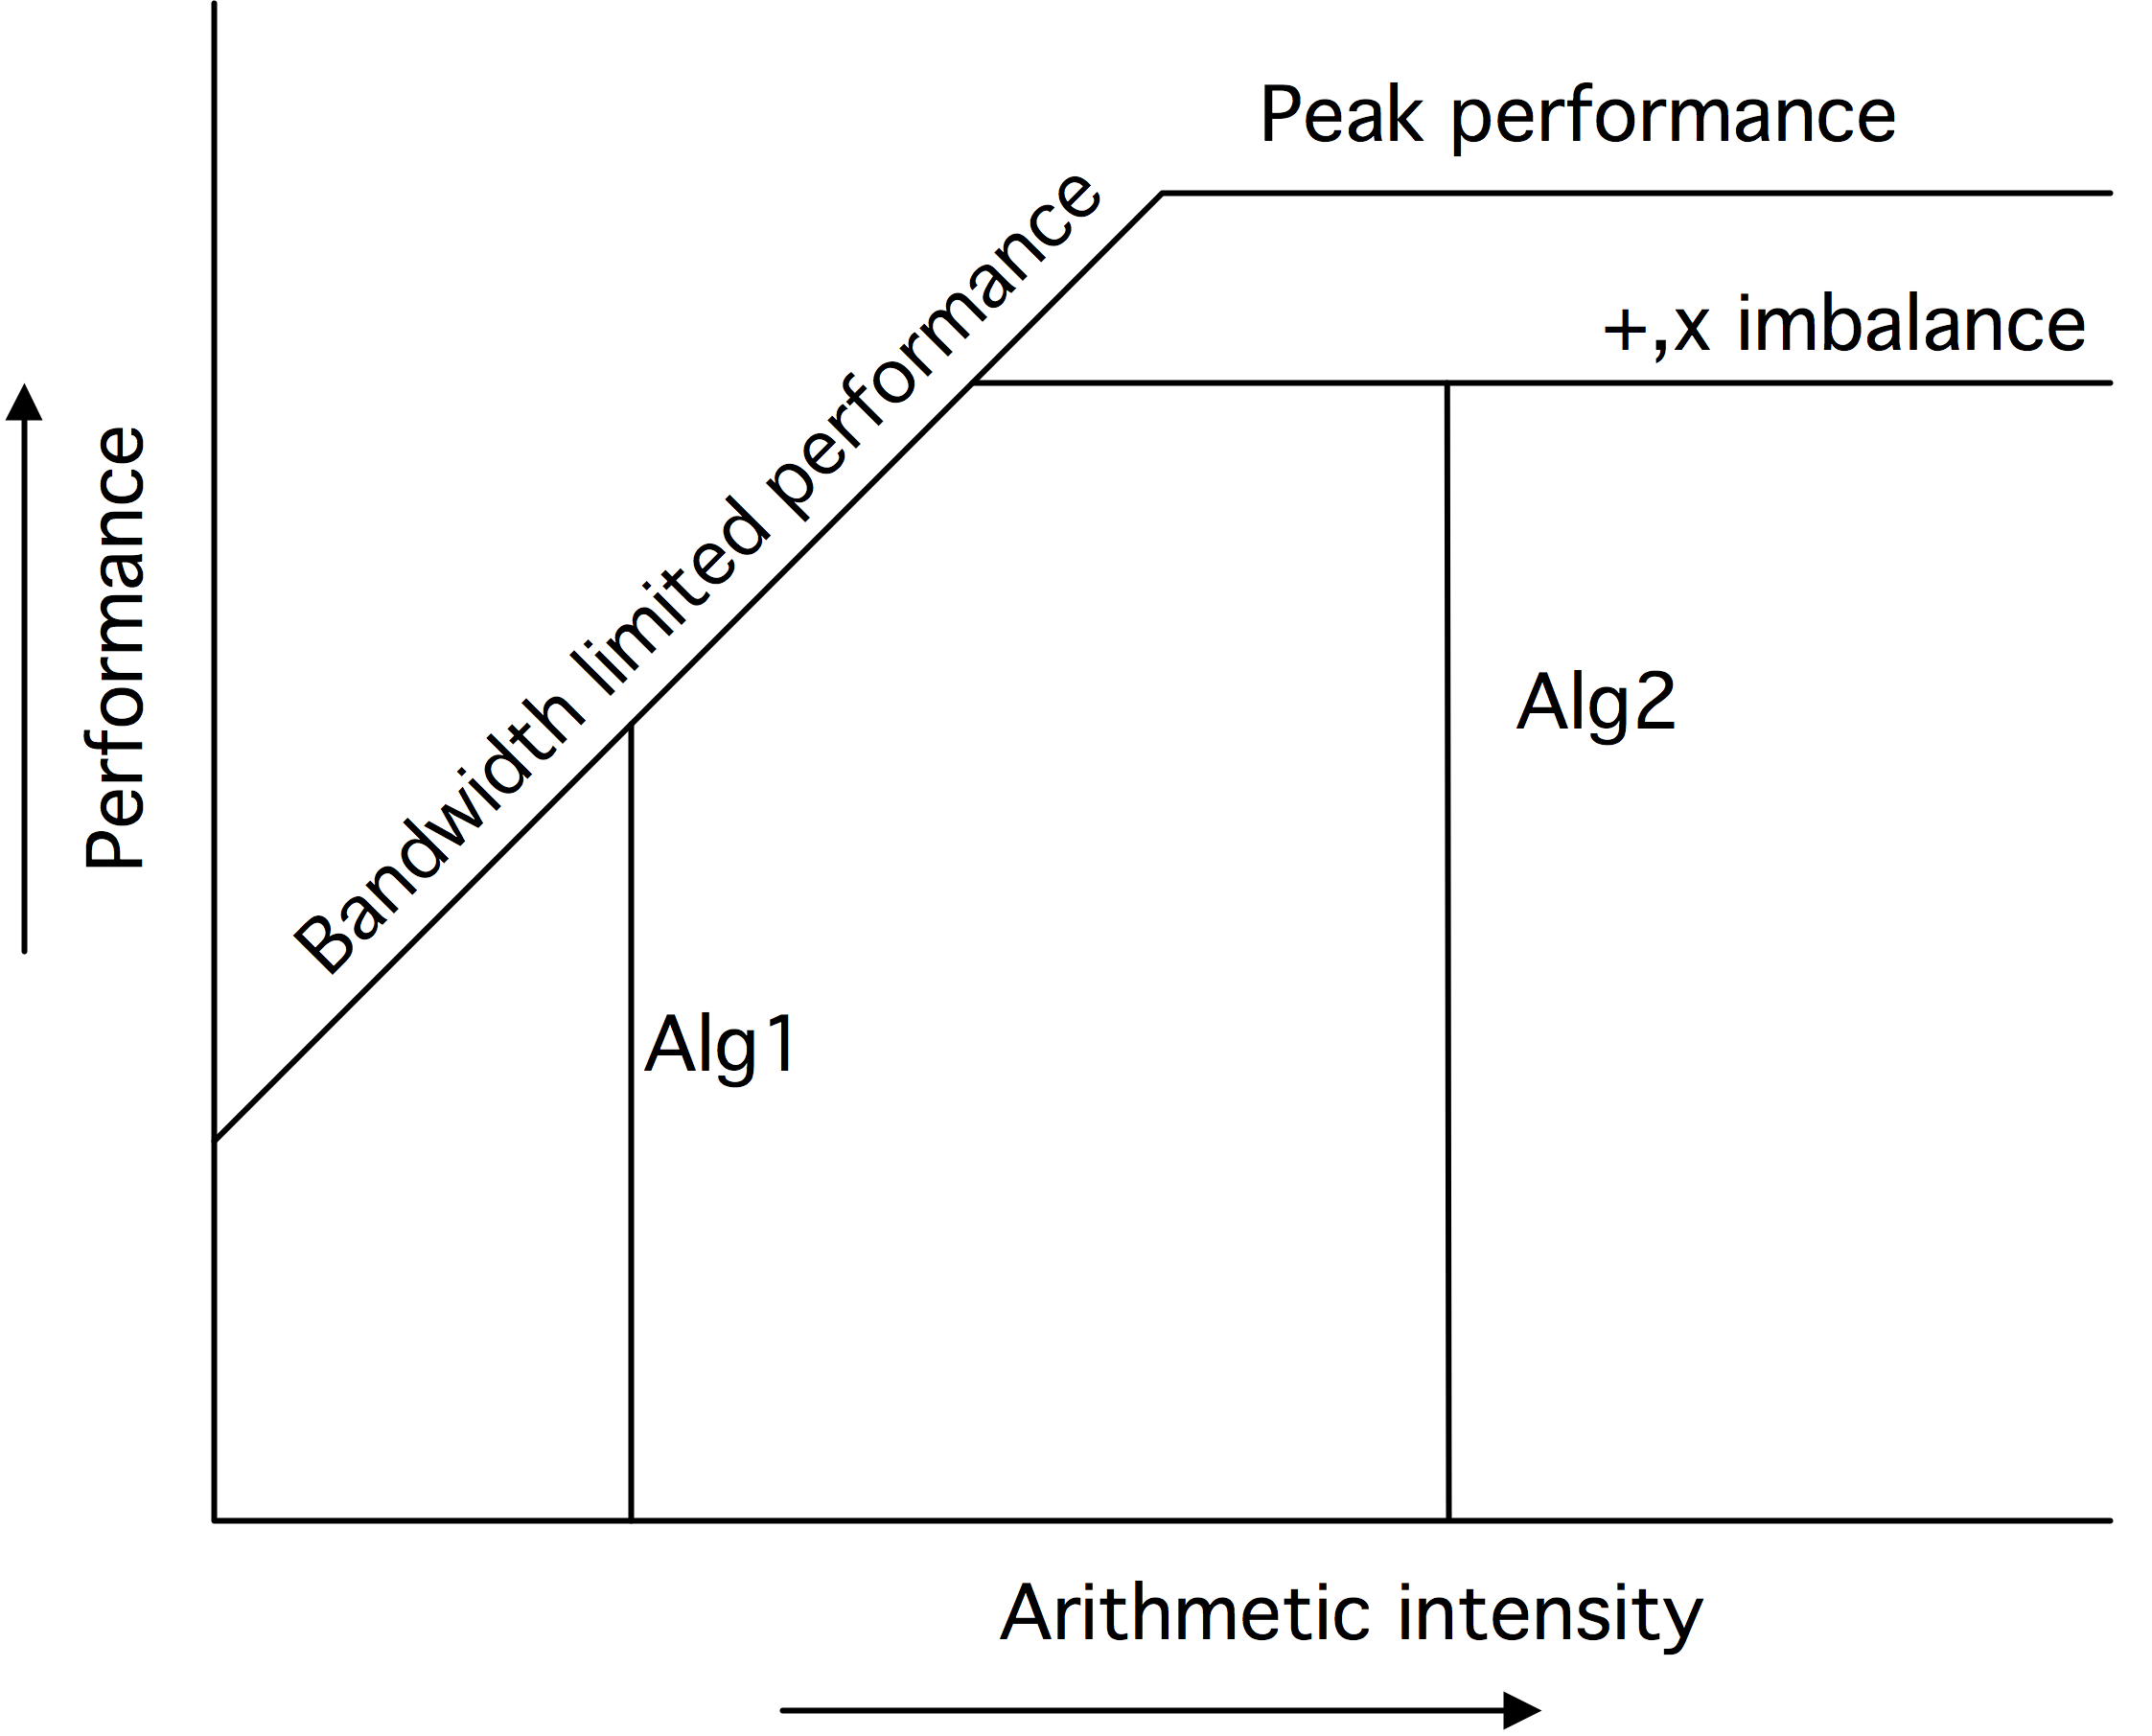
\includegraphics[scale=.1]{graphics/roofline2}
  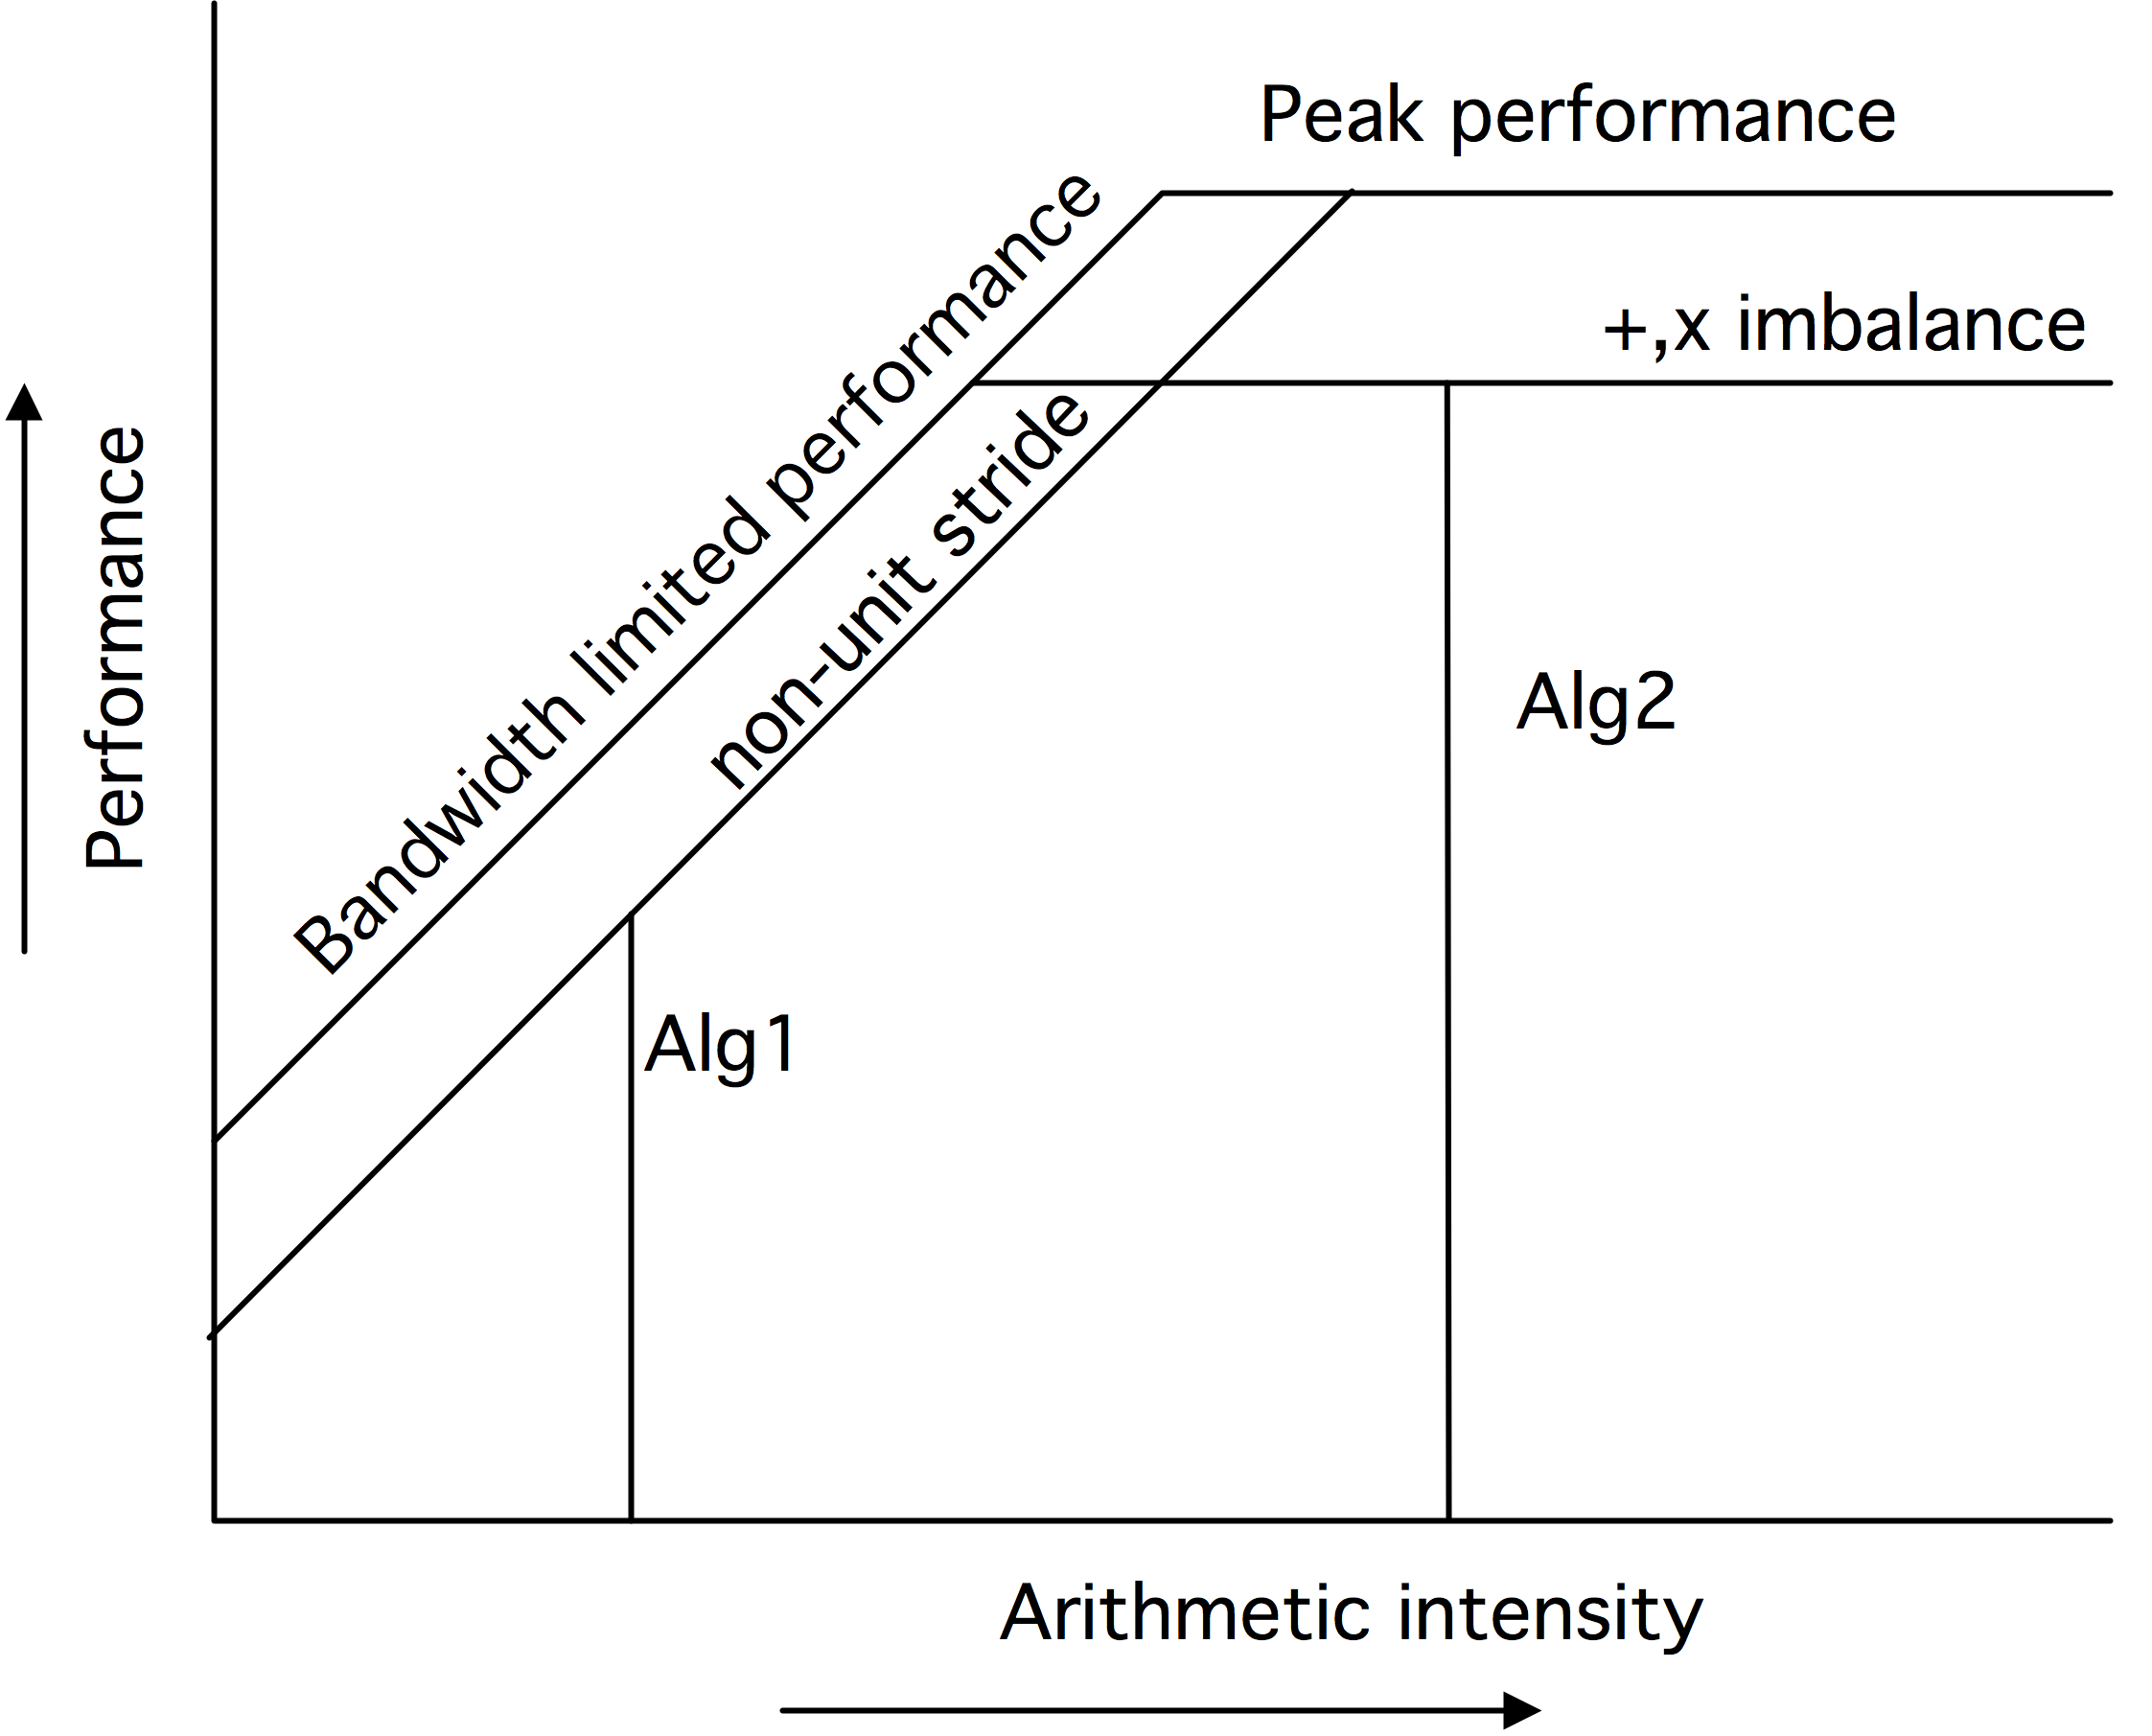
\includegraphics[scale=.1]{graphics/roofline3}

  \caption{Illustration of factors determining performance in the roofline model}
  \label{fig:roofline}
\end{figure}
\begin{enumerate}
\item The \indexterm{peak performance}, indicated by the horizontal
  line at the top of the graph, is an absolute bound on the
  performance\footnote {An old joke states that the peak performance
    is that number that the manufacturer guarantees you will never
    exceed}, achieved only if every aspect of a CPU (pipelines,
  multiple floating point units) are perfectly used. The calculation
  of this number is purely based on CPU properties and clock cycle; it
  is assumed that memory bandwidth is not a limiting factor.
\item The number of operations per second is also limited by the
  product of the bandwidth, an absolute number, and the arithmetic
  intensity:
  \[ \frac{\hbox{\it operations}}{\hbox{\it second}}=
  \frac{\hbox{\it operations}}{\hbox{\it data item}}\cdot
  \frac{\hbox{\it data items}}{\hbox{\it second}}
  \]
  This is depicted by the linearly increasing line in the graph.
\end{enumerate}
The roofline model is an elegant way of expressing that various
factors lower the ceiling.  For instance, if an algorithm fails to use
the full \indextermbus{SIMD}{width}, this inbalance lowers the
attainable peak.  The second graph in figure~\ref{fig:roofline}
indicates various factors that lower the ceiling.
%
There are also various factors that lower the available bandwidth,
such as imperfect data hiding. This is indicated by a lowering of the 
sloping roofline in the third graph.

For a given arithmetic intensity, the performance is determined by
where its vertical line intersects the roof line. If this is at the
horizontal part, the computation is called \indextermdef{compute-bound}:
performance is determined by characteristics of the processor, and
bandwidth is not an issue. On the other hand, if that vertical line
intersects the sloping part of the roof, the computation is called
\indextermdef{bandwidth-bound}: performance is determined by the memory
subsystem, and the full capacity of the processor is not used.

\index{roofline model|)}

\begin{exercise}
  How would you determine whether a given program kernel is bandwidth
  or compute bound?
\end{exercise}

\Level 1 {Locality}
\label{sec:locality}

Since using data in cache is cheaper than getting data from main
memory, a programmer obviously wants to code in such a way that data
in cache is reused. While placing data in cache is not under explicit
programmer control, even from assembly language, in most
CPUs\footnote{Low level memory access can ben controlled by the
  programmer in the Cell processor and in some GPUs.}, it is still
possible, knowing the behaviour of the caches, to know
what data is in cache, and to some extent to control it.

The two crucial concepts here are
\indextermsub{temporal}{locality}\index{temporal
  locality|see{locality, temporal}} and
\indextermsub{spatial}{locality}\index{spatial locality|see{locality,
    spatial}}. Temporal locality is the easiest to explain: this
describes the use of a data element within a short time of its last
use.  Since most caches have a \ac{LRU} replacement policy
(section~\ref{sec:lru}), if in between the two references less data
has been referenced than the cache size, the element will still be in
cache and therefore be quickly accessible. With other replacement
policies, such as random replacement, this guarantee can not be made.

\Level 2 {Temporal locality}

As an example of temporal locality, consider the repeated use of a
long vector:
\begin{verbatim}
for (loop=0; loop<10; loop++) {
  for (i=0; i<N; i++) {
    ... = ... x[i] ...
  }
}
\end{verbatim}
Each element of \texttt{x} will be used 10 times, but if the vector
(plus other data accessed) exceeds
the cache size, each element will be flushed before its
next use. Therefore, the use of \n{x[i]} does not exhibit temporal
locality: subsequent uses are spaced too far apart in time for it to
remain in cache. 

If the structure of the computation allows us to exchange
the loops:
\begin{verbatim}
for (i=0; i<N; i++) {
  for (loop=0; loop<10; loop++) {
    ... = ... x[i] ...
  }
}
\end{verbatim}
the elements of \texttt{x} are now repeatedly reused, and are
therefore more likely to remain in the cache. This rearranged code
displays better
temporal locality in its use of~\n{x[i]}.

\Level 2 {Spatial locality}

The concept of \indextermsub{spatial}{locality} is slightly more
involved. A program is said to exhibit spatial locality if it
references memory that is `close' to memory it already referenced. In
the classical von Neumann architecture with only a processor and
memory, spatial locality should be irrelevant, since one address in
memory can be as quickly  retrieved as any other. However, in a modern CPU
with caches, the story is different. Above, you have seen two examples
of spatial locality:
\begin{itemize}
\item Since data is moved in \indextermbus{cache}{line}s rather than
  individual words or bytes,
  there is a great benefit to coding in such a manner that all
  elements of the cacheline are used. In the loop
\begin{verbatim}
for (i=0; i<N*s; i+=s) {
    ... x[i] ...
}
\end{verbatim}
  spatial locality is a decreasing function of the
  \indexterm{stride}~\n{s}.

  Let \n{S}~be the cacheline size, then as \n{s} ranges from $1\ldots\n{S}$,
  the number of elements used of each cacheline goes
  down from~\n{S} to~1. Relatively speaking, this increases the cost
  of memory traffic in the loop: if $s=1$, we load $1/S$ cachelines
  per element; if $s=S$, we load one cacheline for each element. This
  effect is demonstrated in section~\ref{sec:coding-cacheline}.
\item A second example of spatial locality worth observing involves
  the \ac{TLB} (section~\ref{sec:tlb}). If a program references
  elements that are close together, they are likely on the same memory
  page, and address translation through the TLB will be fast. On the
  other hand, if a program references many widely disparate elements,
  it will also be referencing many different pages. The resulting TLB
  misses are very costly; see also section~\ref{sec:coding-tlb}.
\end{itemize}

\begin{exercise}
  Consider the following pseudocode of an algorithm for summing $n$
  numbers $x[i]$ where $n$ is a power of~2:
\begin{verbatim}
for s=2,4,8,...,n/2,n:
  for i=0 to n-1 with steps s:
    x[i] = x[i] + x[i+s/2]
sum = x[0]
\end{verbatim}
  Analyze the spatial and temporal locality of this algorithm, and
  contrast it with the standard algorithm
\begin{verbatim}
sum = 0
for i=0,1,2,...,n-1
  sum = sum + x[i]
\end{verbatim}
\end{exercise}

\begin{exercise}
Consider the following code, and assume that \n{nvectors} is small
compared to the cache size, and \n{length} large.
\begin{verbatim}
for (k=0; k<nvectors; k++)
  for (i=0; i<length; i++)
    a[k,i] = b[i] * c[k]
\end{verbatim}
How do the following concepts relate to the performance of this code:
\begin{itemize}
\item Reuse
\item Cache size
\item Associativity
\end{itemize}

Would the following code where the loops are exchanged
perform better or worse, and why?
\begin{verbatim}
for (i=0; i<length; i++)
  for (k=0; k<nvectors; k++)
    a[k,i] = b[i] * c[k]
\end{verbatim}
\end{exercise}

\Level 2 {Examples of locality}

Let us examine locality issues for a realistic example. The
matrix-matrix multiplication $C\leftarrow A\cdot B$ can be computed
in several ways. We compare two implementations, assuming that all
matrices are stored by rows, and that the cache size is insufficient
to store a whole row or column.

\hbox{%\begin{quotation}
\setbox0=\hbox{%
\begin{minipage}{.4\textwidth}
\begin{verbatim}
for i=1..n
  for j=1..n
    for k=1..n
      c[i,j] += a[i,k]*b[k,j]
\end{verbatim}
\end{minipage}}
\ht0=1.2\ht0 \box0
\,
\begin{minipage}{.4\textwidth}
\begin{verbatim}
for i=1..n
  for k=1..n
    for j=1..n
      c[i,j] += a[i,k]*b[k,j]
\end{verbatim}
\end{minipage}
}%\end{quotation}
These implementations are illustrated in figure~\ref{fig:ijk-mult}
\begin{figure}[ht]
  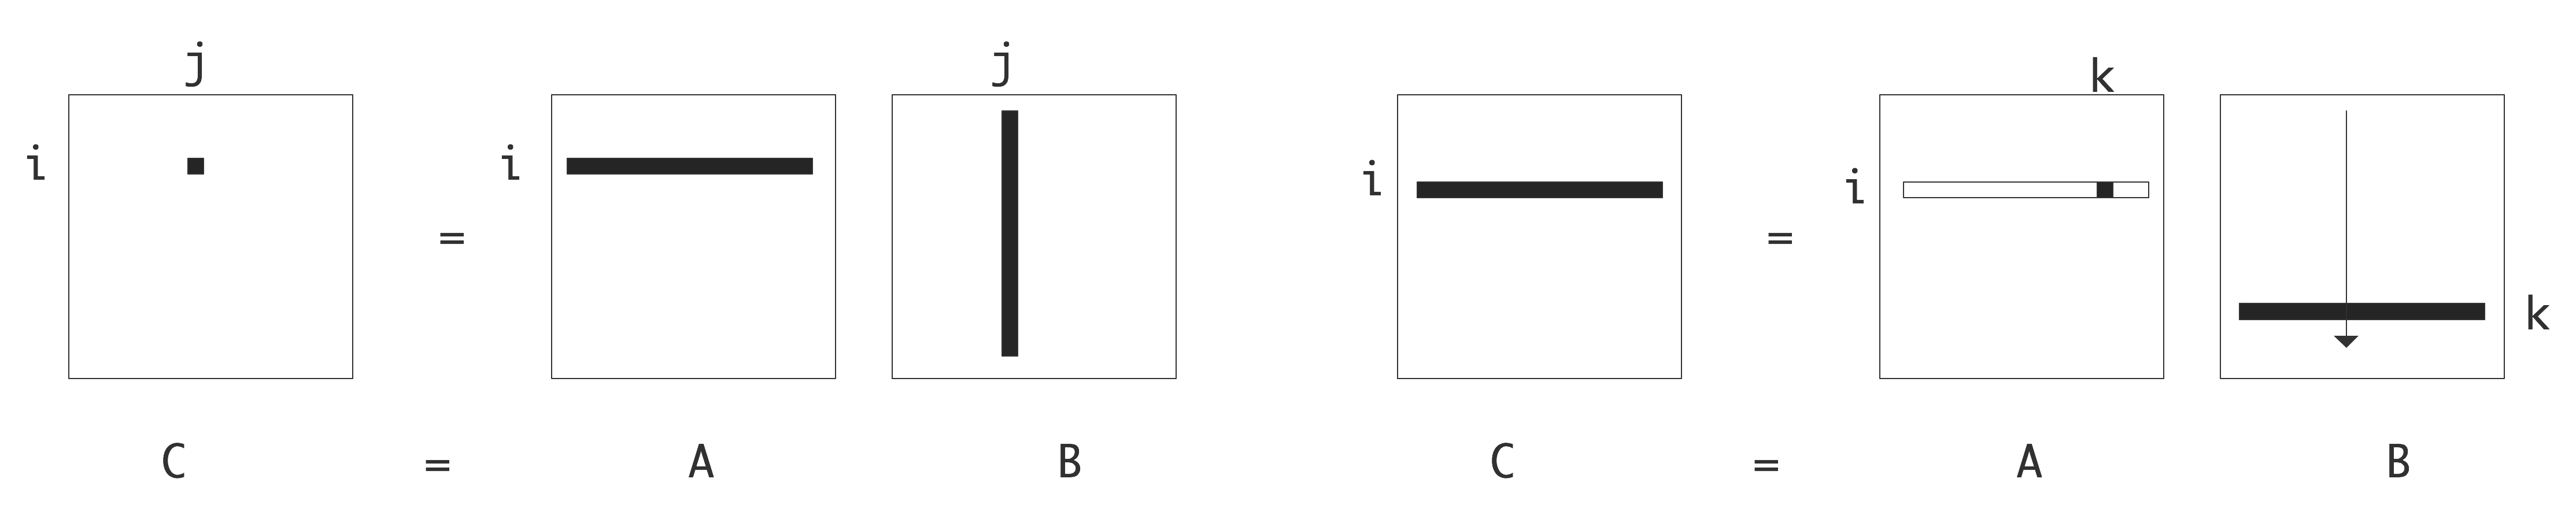
\includegraphics[scale=.1]{graphics/ijk-mult}
  \caption{Two loop orderings for the $C\leftarrow A\cdot B$
    matrix-matrix product}
  \label{fig:ijk-mult}
\end{figure}
The first implemenation constructs the $(i,j)$ element of~$C$ by the
inner product of a row of~$A$ and a column of~$B$, in the second a row
of~$C$ is updated by scaling rows of~$B$ by elements of~$A$.

Our first observation is that both implementations
indeed compute $C\leftarrow
C+A\cdot B$, and that they both take roughly $2n^3$
operations. However, their memory behaviour, including spatial and
temporal locality is very different.
\begin{itemize}
\item[\n{c[i,j]}] In the first implementation, \n{c[i,j]} is
  invariant in the inner iteration, which constitutes temporal
  locality,
  so it can be kept in register. As
  a result, each element of~$C$ will be loaded and stored only once.

  In the second implementation, \n{c[i,j]} will be loaded and stored
  in each inner iteration. In particular, this implies that there are
  now $n^3$ store operations, a~factor of~$n$ more than the first
  implementation.
\item[\n{a[i,k]}] In both implementations, \n{a[i,k]} elements are
  accessed by rows, so there is good spatial locality, as each loaded
  cacheline will be used entirely. In the second implementation,
  \n{a[i,k]}~is invariant in the inner loop, which constitutes
  temporal locality; it can be kept in register. As a result, in the
  second case $A$~will be loaded only once, as opposed to $n$~times in
  the first case.
\item[\n{b[k,j]}] The two implementations differ greatly in how they
  access the matrix~$B$. First of all, \n{b[k,j]}~is never invariant
  so it will not be kept in register, and $B$~engenders $n^3$~memory
  loads in both cases. However, the access patterns differ.

  In second case, \n{b[k,j]}~is access by rows
  so there is good spatial locality: cachelines will be fully utilized
  after they are loaded. 

  In the first implementation, \n{b[k,j]}~is accessed by
  columns. Because of the row storage of the matrices, a cacheline contains
  a part of a row, so for each cacheline loaded, only one element is
  used in the columnwise traversal. This means that the first
  implementation has more loads for~$B$ by a factor of the cacheline
  length. There may also be TLB effects.
\end{itemize}
Note that we are not making any absolute predictions on code
performance for these implementations, or even relative comparison of
their runtimes. Such predictions are very hard to make. However, the
above discussion identifies issues that are relevant for a wide range
of classical CPUs.

\begin{exercise}
  There are more algorithms for computing the product $C\leftarrow
  A\cdot B$. Consider the following:
\begin{verbatim}
for k=1..n:
  for i=1..n:
    for j=1..n:
      c[i,j] += a[i,k]*b[k,j]
\end{verbatim}
Analyze the memory traffic for the matrix~$C$, and show that it is
worse than the two algorithms given above.
\end{exercise}

\begin{comment}
 The following program is likely inefficient if
\texttt{n} is small and \texttt{N} is large:
\begin{verbatim}
for (i=0; i<N; i++)
  for (j=0; j<n; j++)
    ... = ... x[j*N+i] ...
\end{verbatim}
Reversing the loops, when possible, is likely to make the code more
efficient:
\begin{verbatim}
for (j=0; j<n; j++)
  for (i=0; i<N; i++)
    ... = ... x[j*N+i] ...
\end{verbatim}
\end{comment}

\Level 2 {Core locality}

The above concepts of spatial and temporal locality were mostly
properties of programs, although hardware properties such as cacheline
length and cache size play a role in analyzing the amount of
locality. There is a third type of locality that is more intimately
tied to hardware: \indextermsub{core}{locality}.

A code's execution is said to exhibit core locality if write accesses
that are spatially or temporally close are performed on the same core
or processing unit. The issue here is that of
\indextermbus{cache}{coherence} (section~\ref{sec:coherence}) where two
cores both have a copy of a certain cacheline in their local stores.
If they both read from it there is no problem. However, if one of them
writes to it, the coherence protocol will copy the cacheline to the
other core's local store. This takes up precious memory bandwidth, so
it is to be avoided.

Core locality is not just a property of a program, but also to a large
extent of how
the program is executed in parallel.

\Level 0 {Programming strategies for high performance}
\label{sec:performance-programming}
\input chapters/memorycoding

\Level 0 {Power consumption}
\label{sec:power}
\index{power!consumption|(}
\input chapters/power
\index{power!consumption|)}

\begin{notlulu}
\Level 0 {Review questions}

For the true/false questions, give short explanation if you choose the `false' answer.

\begin{exercise}
  True or false. The code
\begin{verbatim}
for (i=0; i<N; i++)
  a[i] = b[i]+1;
\end{verbatim}
touches every element of \n{a} and~\n{b} once, so there will be a cache miss
for each element.
\end{exercise}

\begin{exercise}
  Give an example of a code fragment where a 3-way associative cache will
  have conflicts, but a 4-way cache will not.
\end{exercise}

\begin{exercise}
  Consider the matrix-vector product with an $N\times N$ matrix.
  What is the needed cache size to execute this operation with only
  compulsory cache misses? Your answer depends on how the operation
  is implemented: answer seperately for rowwise and columnwise traversal
  of the matrix, where you can assume that the matrix is always stored by rows.
\end{exercise}
\end{notlulu}

\endinput

\begin{exercise}
  Consider the matrix-vector product operation $y\leftarrow
  Ax$\footnote {The Blas operation for the matrix vector product
    computes $y\leftarrow Ax+y$. The difference in the code involved
    is minimal}:
\begin{verbatim}
for (i<M) {
  s = 0
  for (j<N) {
    s = s + a[i][j] * x[j]; }
  y[i] = s
}
\end{verbatim}
  Can you think of at least one reason why the case $M<N$ would be
  more efficient than $M>N$?
\end{exercise}

exercises:
diagonal format through CRS, why less efficient?

futility of unrolling for memory-bound ops

does manual unrolling help?

Chip power:
\[ P=C_TV_{dd}^2f\gamma \]
where $C_T$ is the effective chip capacitance, $V_{dd}$~is the supply
voltage, $f$~the clock frequency, and $\gamma$~the probability that a
0--1 transition occurs.
Increasing the number of cores increases $C_T$: linear effect.

\[ P=C_TV_{dd}^2f+V_{dd}I_{st}+V_{dd}I_{leak} \]
